\chapter{State of the art}
\label{cha:state-of-the-art}

The emergence of wireless capabilities equipping an ever-growing range of mobile entities has led to various ad hoc\index{Ad hoc networks|bb} paradigms such as \acrfullpl{manet}, \acrfullpl{vanet}\index{Vehicular Ad hoc Network (VANET)|bb}, \acrfullpl{wsn}\index{Wireless Sensor Network (WSN)|bb}, and \acrfullpl{dtn}\index{Delay-Tolerant Network (DTN)|bb}. Various application scenarios were envisioned involving a wide range of entities. Such scenarios include transportation systems and public safety in urban environments or more challenging environments such as remote sensor fields where end-to-end connectivity is not guaranteed. Whereas the common underlying idea to ad hoc networks consists in defining a multi-hop communication path, the main difference in those paradigms lies in how to deal with the mobility of entities and the resulting changes in the topology. 

While mobility is perceived as a problem for \acrshortpl{manet} because it creates connectivity gaps, it is necessary for \acrshortpl{dtn}, which relies on the so-called \textit{store, carry, and forward}\index{Store, carry, and forward} paradigm. Mobile entities then become \textit{data carriers}\index{Data carrier|bb} and are equipped with transmission and storage capabilities, which allows them to carry data and exchange it during an encounter, that is when two entities are in each other's transmission range. The low density of \acrshort{dtn} entities is compensated by a high mobility which allows encounters. Encounters between entities are seen as \textit{opportunities} to forward data across the ad hoc network until eventual delivery. Therefore, instantaneous end-to-end connectivity is not required to route the data, since the data is passed from one entity to the other until it reaches its destination. \Acrshortpl{dtn} involve a broad range of entities either mobile by nature such as humans or animals, or mobile by conception such as vehicles or controllable robots. These entities act as the transportation layer for a wide range of applications, including the collection of data in a sensor fields, bridging connectivity gaps between densely connected regions, and extending the capacity of infrastructure-based networks by providing an alternative transmission medium. The intended application scenarios target specific types of data that can tolerate delay in their delivery. Depending on the entities involved and the application exploiting their movements, the expected benefits depends on various parameters such as the level of knowledge of mobility of the entities, whether their trajectories can be controlled, or the total number of entities involved in the data transfer. These parameters have an impact on the performance metrics we use to compare the different work. These metrics include the delivery ratio (when the data has a timeout), the energy consumption of the entities to transport the data, the delivery delay, and delivery rate.

\begin{figure}
    \centering
    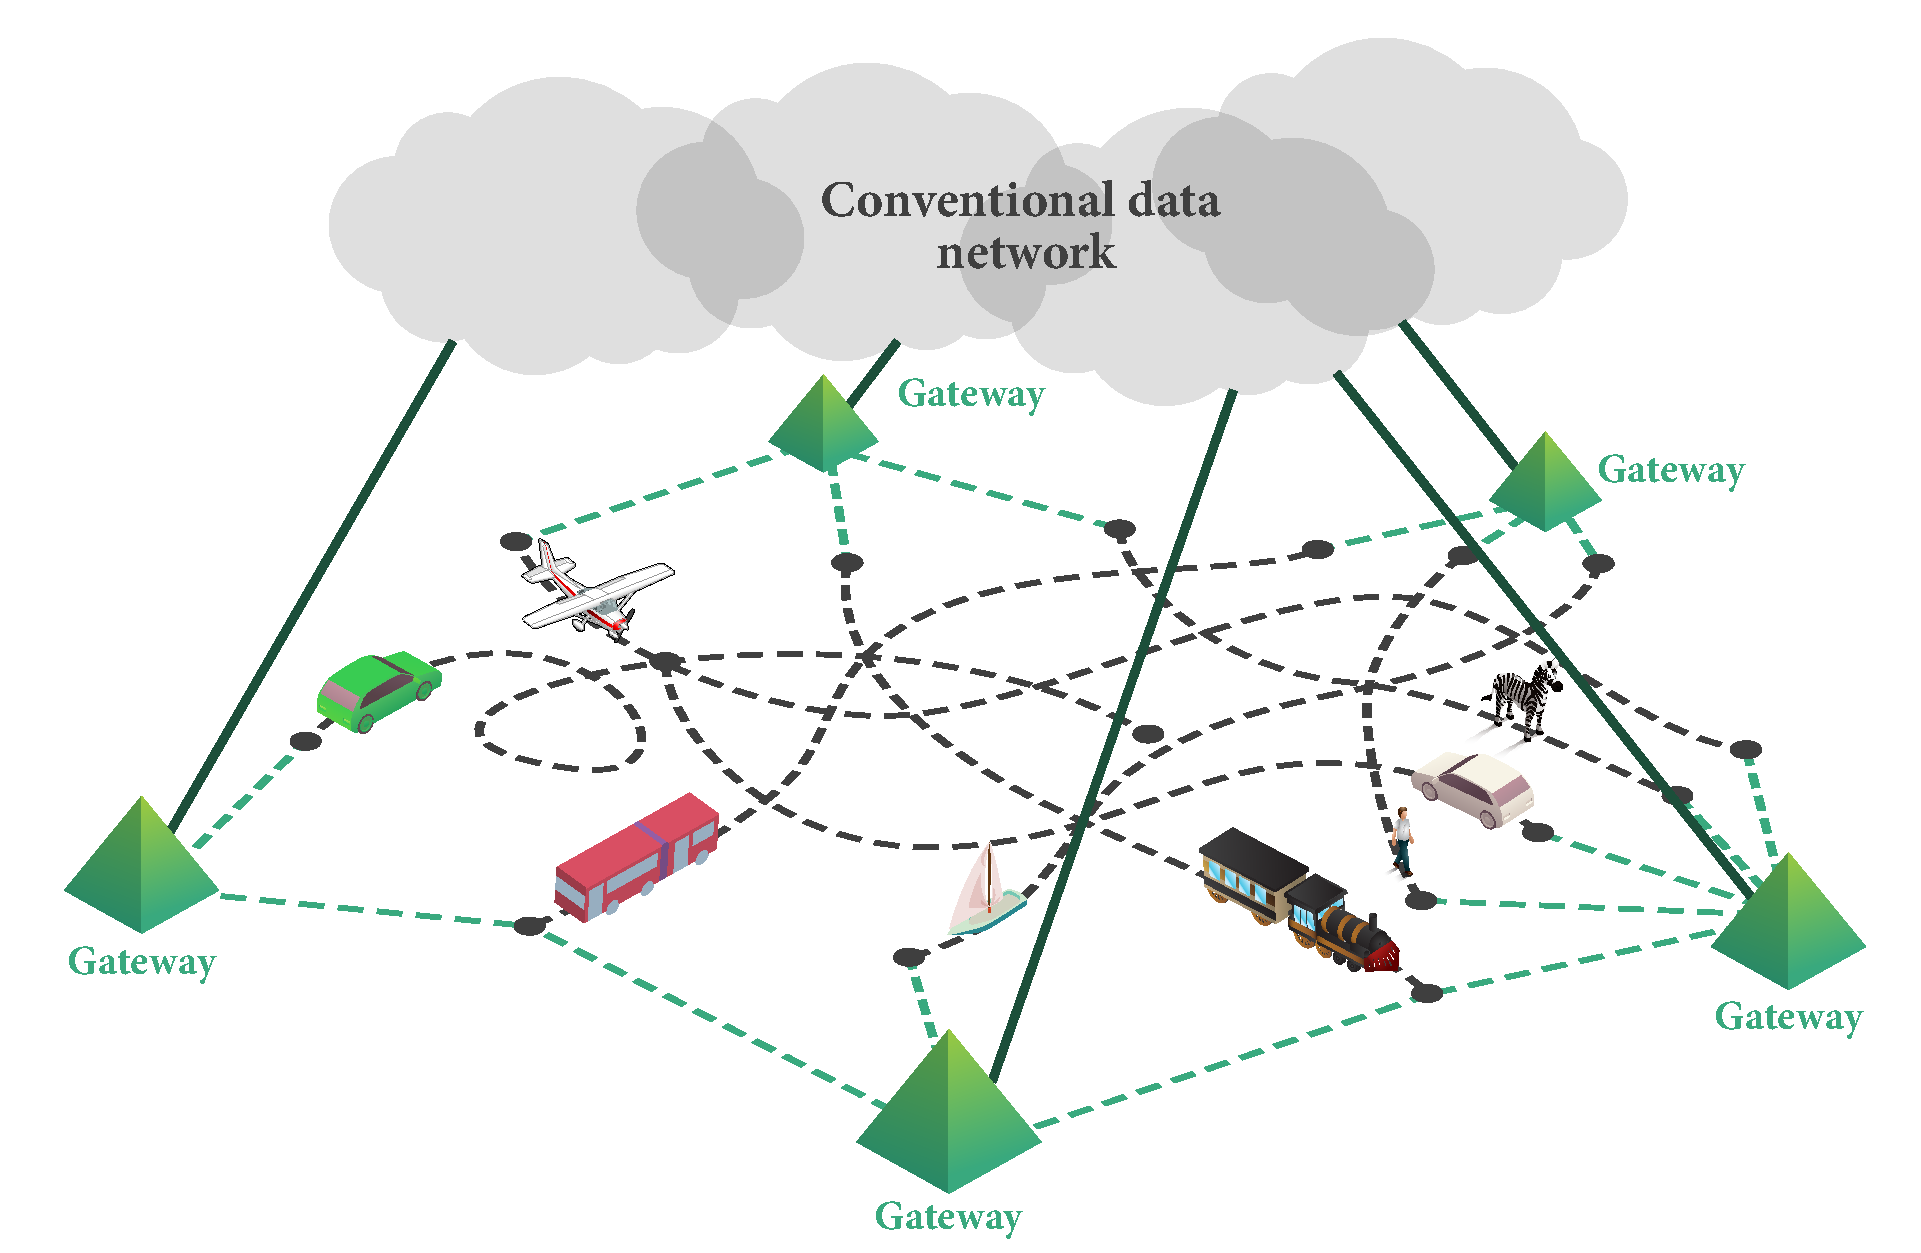
\includegraphics[width=\textwidth]{figures/related-workv2.pdf}
    \caption{Generic architecture for intermodal\index{Intermodal} data transport based on the movements of entities.}
    \label{fig:related-work}
\end{figure}

We represent the generic architecture for such applications in Figure~\ref{fig:related-work}. It includes the movements of entities as transportation layer, and data source(s) and destination(s), that can be connected to infrastructure-based networks such as the Internet. We refer to this generic architecture as \textit{intermodal}\index{Intermodal|bb}, since multiple modes of data transportation are involved to route the data to its destination. In this chapter, we review and provide a comprehensive categorization of the \textit{existing intermodal strategies that leverage different modes of transportation to physically move data}. Most of the approaches exploit the existing mobility of entities to carry data and provide an alternative transmission medium. These entities help deliver data in environments with no computer network available, or as a supplement or replacement to existing computer networks already deployed (\eg to extend their capacities). Therefore, the scope of our study is not limited to the opportunistic approaches that rely on the movements of the entities, as we also review offloading techniques seeking for cost-effective solutions to extend the capacity of infrastructure-based networks. The main contribution of the work we review lies in their approaches to alleviate the limited control over the lack of knowledge of the mobility of the entities when they move for other purposes than the intended data transport. 

The simpler approach is to use a single entity that will eventually make the entire trip between the source(s) and the destination(s) of the data transfer. However, the opportunistic movements of these entities cannot be predicted and do not necessary match the source(s) and destination(s) of the data transfers. As a result, there are no guarantees on the actual delivery of data. This approach is well-suited for large-scale sensing applications that cover large areas. However, with some knowledge on the mobility of the entities (\eg bus movements between cities), one can exploit the structure present in their movements to transfer data over larger distances and provide better guarantees on the data transfers in terms of achievable throughput and delivery delay. The approach followed by delay-tolerant networks consists in combining the trajectories of the entities and relay the data from one entity to the other to its destination~\cite{fall2003delay}. The main problem these approaches address is whether to forward a data during this encounter or carry it instead. While these approaches can act as a transportation layer, they all assume a standalone network with transfers from one entity to another. Since our focus here is the intermodal approaches, the \acrshort{dtn} approaches do not fall within our scope. However, we refer the reader to the following surveys on the different routing strategies in \acrlongpl{dtn}:~\cite{zhang2006routing,spyropoulos2010routing,khabbaz2012disruption,pereira2012delay}. Approaches proposed to deploy support transport infrastructures that enable data relaying between entities. As part of the deployed infrastructure, dedicated nodes, either mobile or fixed, capture the trajectories of the entities and temporarily store the data to transfer until other entities meet them. Finally, while the existing mobility of entities can be used opportunistically to transport data, other approaches proposed to rely on third-party services to transport the data over large distances, such as postal services (\eg FedEx, UPS or USPS). These services manage entities of their own to provide guarantees (in terms of cost and delay) to transport the data contained in parcel to its destination. 

% \section{Classification}

% \begin{wrapfigure}[12]{o}[0.7\marginparwidth]{6.5cm}
%     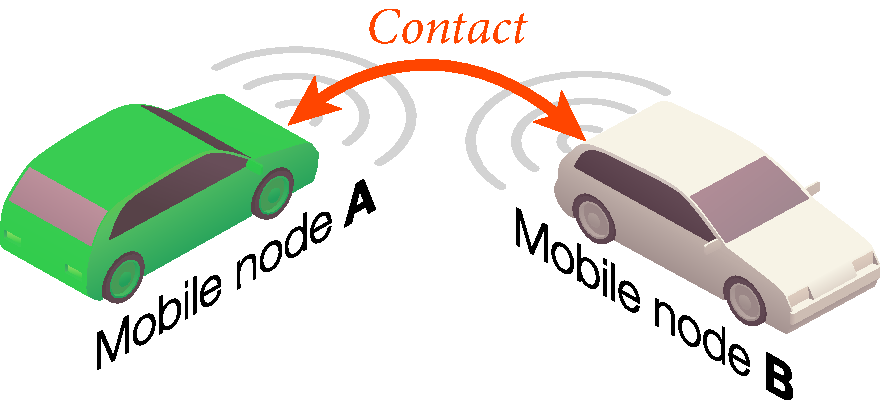
\includegraphics[width=6cm]{figures/dtn-routing.pdf}
%     \caption{Example of DTN routing between two mobile nodes. The contact happens whenever the two nodes are in each other's transmission range.}
%     \label{fig:dtn-routing}
% \end{wrapfigure}

% Define: mobility structure, data carriers, contact, entities, infrastructure

% In this survey, we focus on the \textit{mobility structure of the entities}, which can be categorized at a high level according to the different levels of knowledge on the mobility of the entities under consideration. This factor is the most important when it comes to transfer data as part of end-to-end services on top of such networks. The simpler case is to use the entities that will eventually make the entire trip between the source and the destination of the data transfer. However, the opportunistic movements of the entities cannot be predicted and will not necessary match the sources and destinations of the data transfers. As a result, there is no guarantees on the actual delivery of data. With some knowledge on the mobility of the entities, one can exploit the structure present in the movements of the entities. This allows to combine the trajectories of the entities, which take turns to \textit{relay the data} towards its destination. Adapting the movements of the entities to the transfer requirements allows better utilization of the ``carry'' phase of the entities. Approaches proposed to deploy infrastructures that enable the data relay between entities. As part of the deployed infrastructure, dedicated nodes, either mobile or fixed, capture the trajectories of the entities and temporarily store the data to transfer until other entities meet the dedicated nodes. Other approaches proposed to relay the data when the entities come in contact\index{contact}, that is, when the entities are within each other's transmission ranges. These contacts are considered as \textbf{opportunities} to relay data and bring it closer to its destination. These approaches propose algorithms that determine whether the entity in contact is suitable to transport the data towards its destination. While the existing mobility of entities can be used to opportunistically transport data, other approaches proposed to use third-party services to transport the data over large distances, such as postal services (\eg FedEx, UPS or USPS). These services manage entities of their own to provide guarantees (in terms of cost and delay) to transport the data contained in parcel to its destination. 

% In this survey, we focus on \textit{how} the entities deliver the data to its destination(s). Over the course of a transfer, either a single entity or multiple entities can relay each other to carry the data to its destination. The data delivery can be categorized at a high level according to whether a single entity or multiple entities are involved in the data transfer. The resulting data transfers will then be delivered either directly by a single entity or relayed by multiple entities that take turns to carry the data towards its destination(s). We represented this classification according to the type data delivery in Figure~\ref{fig:classification-survey}.

\begin{figure}[!h]
\centering
\resizebox{0.9\textwidth}{!}{%
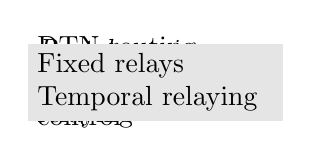
\begin{tikzpicture}[every tree node/.style={align=center,anchor=north},level 1/.style={level distance=1.5cm},level 2/.style={level distance=2cm}]
\Tree [.\textbf{Data delivery} 
        [.{\textbf{Direct} delivery\\Single entity}
            [.\node[text width=3cm]{\textit{Data MULEs}\\No control}; ] 
            [.\node[text width=3cm]{\textit{Postal services}\\Source/Destination control}; ]
            [.\node[text width=3cm]{\textit{Robots}\\Trajectory control}; ] ] 
        [.{\textbf{Indirect} delivery\\Multiple entities} 
            [.\node[text width=3cm]{DTN routing\\Spatial/temporal relaying}; ] 
            [.\node[text width=3cm]{Mobile relays\\Spatial relaying}; ] 
            [.\node[draw=gray!20,text width=3cm,fill=gray!20]{Fixed relays\\Temporal relaying}; ] ] ]
\end{tikzpicture}}
\caption{Classification according to the type of data delivery.}
\label{fig:classification-survey}
\end{figure}

\begin{figure}[!h]
\centering
\resizebox{0.95\textwidth}{!}{%
\begin{tikzpicture}[every tree node/.style={align=center,anchor=north},level 1/.style={level distance=1.5cm},level 3/.style={level distance=1.5cm}]
\Tree [.\textbf{Data carrier mobility} 
        [.{\textbf{Controllable} mobility} 
            [.{Mobility designed\\for data transport} 
                [.{Static\\trajectory} ]
                [.{Dynamic\\trajectory} ] ] 
            [.{Third-party\\services} ] ] 
        [.{\textbf{Non-controllable} mobility} 
            [.{With fixed\\infrastructure} ] 
            [.{Without fixed\\infrastructure}
                [.{End-to-end\\delivery} ]
                [.{Multi-hop\\delivery} ] ] ] ]
\end{tikzpicture}}
\caption{Classification according to the data carrier mobility}
\label{fig:classification-survey}
\end{figure}

\begin{figure}[!h]
\centering
\resizebox{0.95\textwidth}{!}{%
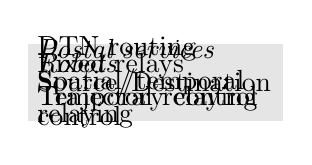
\begin{tikzpicture}[every tree node/.style={align=center,anchor=north},level 1/.style={level distance=1.5cm},level 4/.style={level distance=1.5cm}]
\Tree [.\textbf{Mobility of the entities} 
        [.{\textbf{No control} over the mobility}
            [.{\textbf{Without} structure} {Data MULES} Epidemic ]
            [.{\textbf{With} mobility structure}
                [.{\textbf{With} dedicated\\infrastructure} 
                    [.\node[text width=3cm]{Mobile relays\\Spatial relaying}; ] 
                    [.\node[draw=gray!20,text width=3cm,fill=gray!20]{Fixed relays\\Temporal relaying}; ] ]
                [.{\textbf{Without} dedicated\\infrastructure} \node[text width=3cm]{DTN routing\\Spatial/temporal relaying}; ]  ] ] 
        [.{\textbf{Control} over the mobility} 
            [.\node[text width=3cm]{\textit{Postal services}\\Source/Destination control}; ] 
            [.\node[text width=3cm]{\textit{Robots}\\Trajectory control}; ] ] ]
\end{tikzpicture}}
\caption{Classification according to the data carrier mobility}
\label{fig:classification-survey}
\end{figure}

\begin{figure}[!h]
\centering
\resizebox{0.95\textwidth}{!}{%
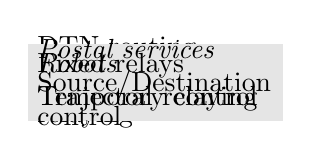
\begin{tikzpicture}[every tree node/.style={align=center,anchor=north},level 1/.style={level distance=1.5cm},level 2/.style={level distance=1.5cm}]
\Tree [.\textbf{Data transport} 
        [.{\textbf{Opportunistic}\\data transport}
            [.{\textbf{Without} mobility structure} {Data MULES\\Epidemic} ]
            [.{\textbf{With} mobility structure}
                [.\node[text width=3cm]{DTN routing\\Spatial/temporal relaying}; ]  ] ]
        [.{\textbf{Support} with dedicated\\infrastructure} 
            [.\node[text width=3cm]{Mobile relays\\Spatial relaying}; ] 
            [.\node[draw=gray!20,text width=3cm,fill=gray!20]{Fixed relays\\Temporal relaying}; ] ]
        [.{\textbf{Full dedicated}\\infrastructure} 
            [.\node[text width=3cm]{\textit{Robots}\\Trajectory control}; ]
            [.\node[text width=3cm]{\textit{Postal services}\\Source/Destination control}; ] ] ]
\end{tikzpicture}}
\caption{Classification according to the data carrier mobility}
\label{fig:classification-survey}
\end{figure}

\begin{figure}[!h]
\centering
\resizebox{0.8\textwidth}{!}{%
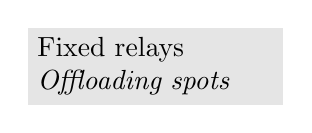
\begin{tikzpicture}[every tree node/.style={align=center,anchor=north},level 1/.style={level distance=1.5cm},level 2/.style={level distance=1.5cm},level 3/.style={level distance=1.5cm}]
\Tree [.\textbf{Intermodal data transport} 
        [.{Opportunistic\\data transport}
            [.{Sensing\\platforms} ]
            [.{Large-scale\\transfers} ] ]
        [.{Support transport\\infrastructure} 
            [.{Tailored transport\\infrastructure}
                [.\node[text width=3cm]{Mobile relays\\\textit{Ferries}}; ] 
                [.\node[draw=gray!20,text width=3cm,fill=gray!20]{Fixed relays\\\textit{Offloading spots}}; ] ]
            [.{Existing transport\\infrastructure} {Postal services} ] ] ]
\end{tikzpicture}}
\caption{Classification according to the intermodal data transport}
\label{fig:classification-survey}
\end{figure}


% In the first case, a single entity is in charge of transporting the data from its source delivering it directly its destination. Such an entity can be used to collect sensor data in a sparse sensor network or send large amounts of data over long distances. This approach is generally known as ``Data MULE''\index{Data MULE} in the literature, which stands for Mobile Ubiquitous LAN Extensions. The mobility of the data carrier can be only known by the service provider, which will match the opportunistic movements of the entity with the sources and destinations of the data transfers to set up. Note that the service providers does not know for sure whether the entity will eventually visit the sources or the destinations and thus cannot provide any guarantees on the performance of the data transfer. Postal services such as FedEx, UPS or USPS can be seen as a single entity and allow the service provider to send large amounts of data directly in parcels over large distances. While the service provider controls the source and destination of the data transfers, providing services with multiple sources or destinations such as sensor data collection remain impossible. Vehicles that are part of a dedicated fleet or mobile robots allow more flexibility when collecting and transferring the data. The service provider has full control over the data carriers and supervises the the origins(s), destination(s), and entire trajectory of the data carriers such that it matches the requirements of the service to provide.

% In the second case, multiple entities are in charge of transporting the data from its source to its destination. The entities we consider move as usually and do not modify their trajectories to adapt it to the data transfers. With the Delay-Tolerant Networking (DTN) parading, the mobile entities are expected to exchange data when in each others' transmission ranges. These meetings are considered as  \textbf{opportunities} to relay data and bring it closer to its destination. Since the movements of the mobile entities have some degree of randomness, the service provider cannot provide any guarantees on the actual delivery of the transfer, as with the case of Data MULEs and a single entity. To this end, a large body of work was done in the fields of DTNs to have efficient routing algorithms that try to make the best use of the meeting opportunities among the mobile entities. Since a large number of surveys were done about this field, we will not survey all the approaches here. Instead, we refer the reader to the following surveys: \cite{pereira2012delay,zhang2009routing,khabbaz2012disruption}. DTN routing protocols require the two meeting entities to be temporally and spatially synchronous to exchange the data to one another. This is a strong assumption, especially for networks that show sparse connectivity and where mobile entities rarely meet one another. Other approaches were proposed to overcome this assumption and propose to use a dedicated infrastructure that allows to asynchronously exchange data between entities. The first infrastructure that was proposed in the literature is the use of dedicated vehicles that either have static or dynamic routes. This allows other mobile entities to meet the vehicles on their route to exchange data. Alternatively, the vehicles can meet the entities on request. The second infrastructure consists of placing fixed nodes equipped with data storage to relay data from one entity to another. These nodes are placed at strategic locations such that they capture the trajectories of a large number of entities going in different directions. The work we present in this thesis is included in the latter approach. The offloading spots we use to temporarily store data dropped off by vehicles allows to relay this data between flows of vehicles going in different directions. The use of these relay nodes allows to avoid solely rely on vehicles making trips all the way from the source to the destination of data.


\section{Taxonomy: Opportunistic data transport}
\label{sec:opportunistic-data-transport}

In this section, we review the \textit{opportunistic use} of data carriers to transport data to its destination. We first review the seminal work on the opportunistic use of mobile entities to transport data. Second, we review the work  that leverage the mobility of various entities to collect sensing data as part of sensing platform that monitor the environment. Finally, we review the work that take into account the structure in the mobility patterns of the entities to achieve large-scale transfers between remote area. 
% With multiple entities, the entities can communicate with one another when in each others' communication range. Replicating the data when encountering another entity allows to improve the overall network performance in terms of latency. However, this technique has a large overhead. More efficient routing techniques are possible when the movements of the entities show periodic patterns. This allows to collect and use statistics to make informed forwarding decisions when two entities are in contact.


\subsection{Background on the opportunistic use of entities as data carriers}

We review the seminal work that exploit the random movements of entities to carry data and transfer it to its destination. These various approaches serve as a basis for the work we will review in the following.

\begin{wrapfigure}[9]{o}[0.7\marginparwidth]{6.3cm}
    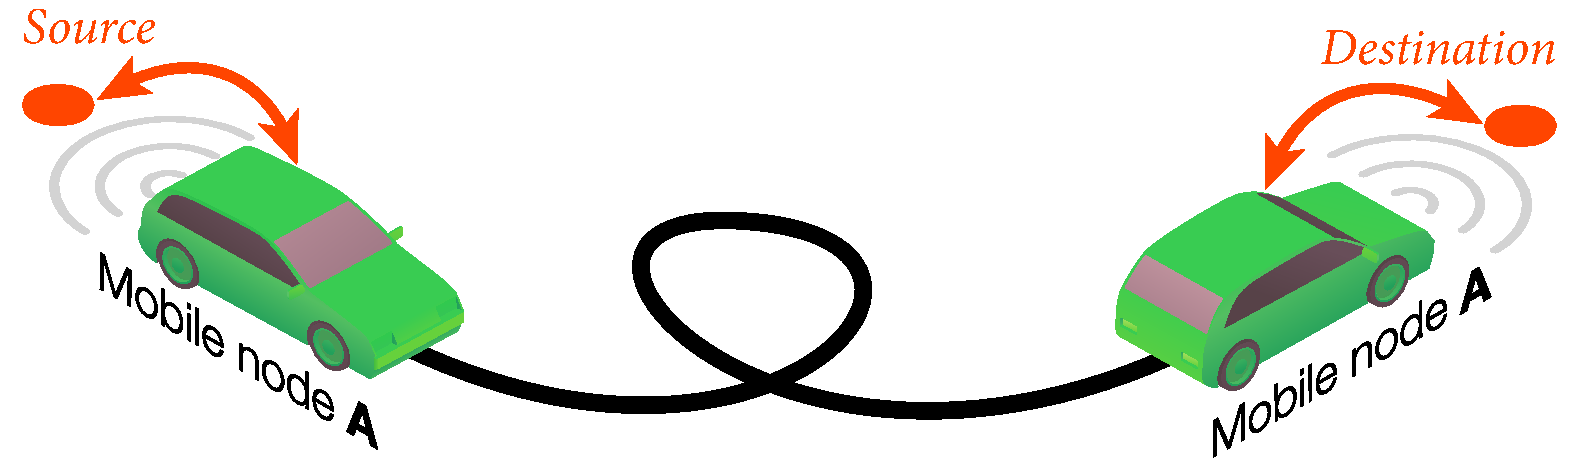
\includegraphics[width=6cm]{figures/direct-delivery.pdf}
    \caption{Example of the direct delivery routing protocol.}
    \label{fig:direct-delivery}
\end{wrapfigure}
In the simplest case, a single entity is in charge of picking up the data at the source and eventually delivering it at its destination. Since only one copy of the data is carried, this approach does not consume many resources and has a minimum overhead\index{Routing!Direct delivery}. However, there are no guarantees on the expected delivery, which makes this strategy highly unreliable. Grossglauer and Tse propose a theoretical model of an ad hoc network with mobile entities~\cite{grossglauser2001mobility}. In particular, they study the benefits of using the mobility of the entities to relay data from its source to its destination. The authors compare their approach to a traditional ad hoc networks where the throughput decreases as the number of nodes increases. Indeed, most of the traffic carried by the entities is relayed traffic, which results in low throughput per pair (source, destination) and high energy consumption. With the model of mobile nodes proposed by the authors, every entity gets close to any other entity for some time. Using a single entity as relay is therefore sufficient to deliver the data to its destination, even though the delivery delay is averaged over long duration. Since the authors assumed a complete mixing of trajectories where any entity can get close to any other, this model sets a theoretical upper bound in the throughput.

\begin{figure}
    \centering
    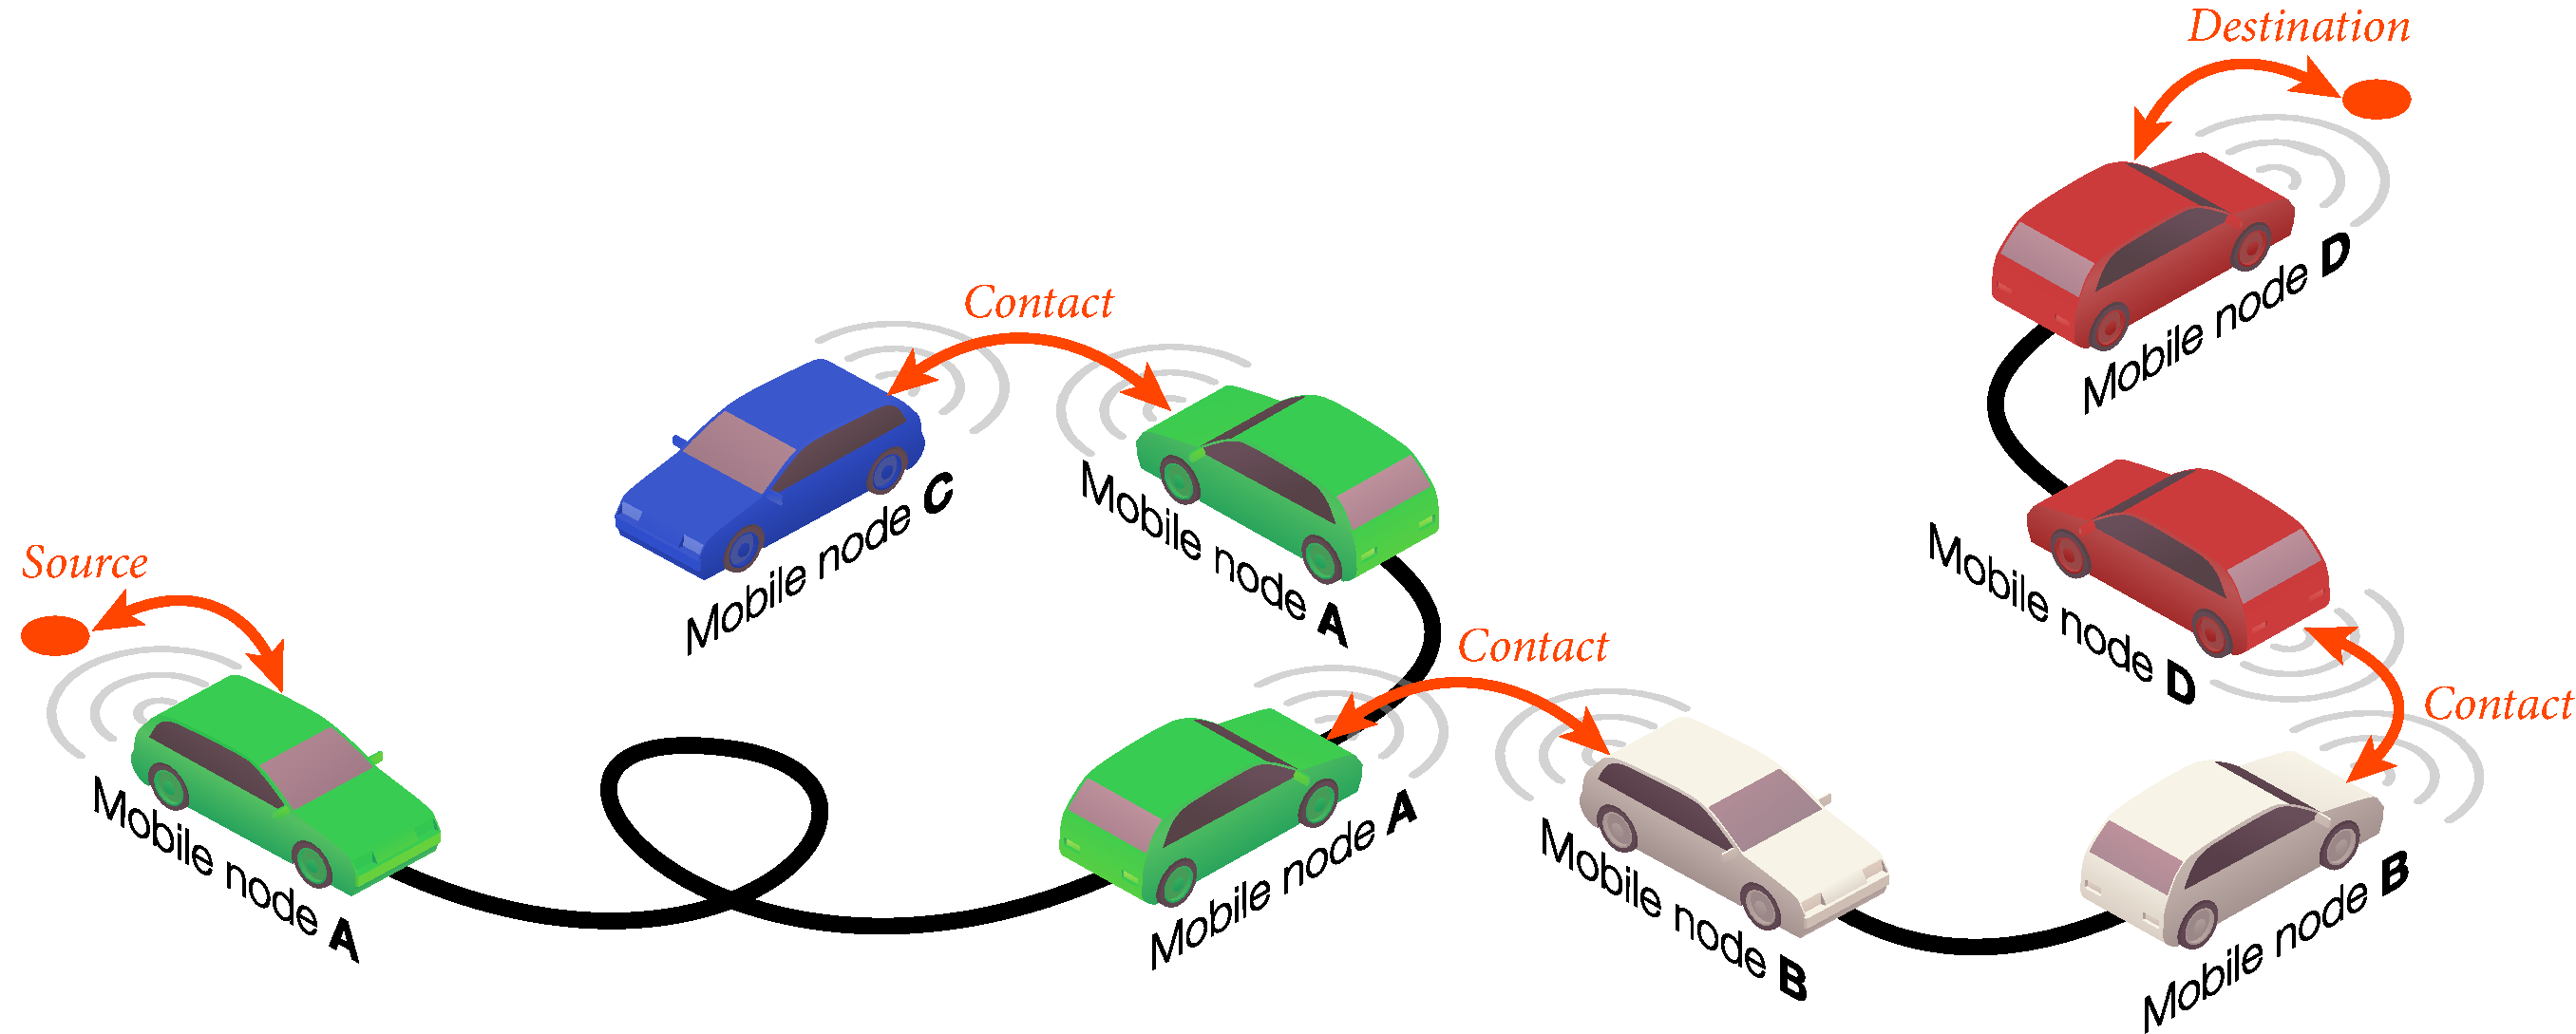
\includegraphics[width=0.7\textwidth]{figures/epidemic.pdf}
    \caption{Example of the Epidemic routing protocol with four mobile nodes.}
    \label{fig:epidemic-protocol}
\end{figure}

With the previous strategy, the delivery delay of the messages may prove to be large if the entity relaying the data takes some time before meeting the destination. On the other side of the spectrum, Vahdat and Becker propose an epidemic routing\index{Routing!Epidemic} protocol that disseminates the data to all the entities the source meets~\cite{vahdat2000epidemic}. Every intermediate entity that receives the data replicates it to all its neighbors and so on. With this approach, the data is certain to be delivered with the minimum delay at its destination, as one of the copies follows the shortest path between the source and the destination. However, replicating the data incurs a large overhead and high consumption of resources, which is not suitable in a mobile environment with limited resources.

These two strategies show the performance trade-off there is in such networks. The goal is to minimize the delivery \textit{delay} of the data, while maximizing the resulting \textit{capacity}. Collaboration among the entities to relay the data to its destination is then necessary. This is the approach followed by most \acrshort{dtn} routing techniques\index{Routing!DTN}. These techniques rely on replications strategies to help decrease the delivery delay by offering more possible paths to the data destination. However, using excessive replication incurs a large overhead and high utilization of the resources of the entities, including local storage and processor. Approaches in the DTN literature aim to reduce the overhead of the replication by either deleting the remaining copies once one copy of the data has been delivered~\cite{balasubramanian2007dtn,juang2002energy}, or by bounding the number of copies replicated~\cite{spyropoulos2005spray,harras2005delay}. Another way to reduce the replication is to use probabilistic routing based on weights assigned to the entities that represent the suitability of the entities to deliver the data to a given destination~\cite{davis2001wearable,burgess2006maxprop,lindgren2003probabilistic,davis2001wearable,burns2005mv,juang2002energy}.

% from https://uwspace.uwaterloo.ca/bitstream/handle/10012/814/ejones2006.pdf?sequence=1

% Spray and Wait [23] protocol is a multi-copy routing protocol
% that controls the flooding overhead by limiting the number of
% message copies distributed in the Spraying phase and then
% relies on direct delivery when a message is transmitted to
% the final destination, then waits until the destination meets
% one of them. Harras et al. (Delay
% tolerant mobile networks (DTMNs): Controlled
% flooding schemes in sparse mobile network) have improved and evaluated
% the controlled message flooding schemes with heuristics,
% for instance, on hop limits or timeouts. Approaches
% falling into this category usually distribute multiple copies
% in the network, to ensure a high reliability of delivery and a
% low latency. But they also bring in a high price of the buffer
% occupancy and bandwidth consumption.


\subsection{Large-scale opportunistic data transfers}

Several approaches propose to leverage the existing movements of mobile entities such as buses~\cite{pentland2004daknet}, cars~\cite{tan2014vehicular}, airline passengers~\cite{keranen2009dtn} to transport data over large distances. As an example, these large-scale intermodal transfers allow extending the connectivity of remote areas not covered by infrastructure networks. The data is loaded in the storage devices carried by the mobile entities when they come close to a source gateway (generally connected to an infrastructure network). The entities then transport the data as part of their normal movements, and unload the data when they come close to a destination gateway. Note that the data can be forwarded from one entity to another to avoid the need to rely on one entity making the entire trip from the source gateway to the destination gateway. Relying on entities with periodic movements such as buses allows to give guarantees on the data transfers (\eg in terms of delivery delay).

DakNet\index{DakNet|bb} is a system offered by First Mile Solution that was deployed on buses in remote parts of India and Cambodia~\cite{pentland2004daknet}. The name comes from Hindi ``Dak'' that means post or postal. The system brings Internet connectivity to the remote regions by taking advantage of the existing bus transportation infrastructure to carry data from a central Internet access point (located in a large city) to remote villages. To this end, Mobile Access Points (MAPs) are mounted on buses or motorbikes that regularly visit villages. Through the MAPs, the mobile entities physically transport the data between the villages and the Internet access point. The MAPs come in contact with kiosks located in the villages and drop off or pick up data from the kiosk. The authors were able to achieve data transfers of 20~MB on average over one contact, either in upload or download. With this system, populations living in the remote villages can be connected to the Internet, as well as other villages. However, they can only exchange non-interactive delay-tolerant data, such as mail or land records. The authors implemented the system on buses that run six times a day to the remote villages of the region of Bhoomi in India. In particular, they detail the low cost of the deployment, and the good reception by villagers, who avoid making long and expensive trips to the main city to obtain land records.

Multiple similar initiatives have been proposed following the DakNet model. The Wizzy Digital Courier service provides connectivity to access schools located in remote villages of South Africa~\cite{rabagliati2004wizzy}. KioskNet is a generic architecture for distributed applications that tolerate large delays~\cite{seth2006low,guo2007very,guo2011design}. Since the system relies on the rural kiosks to forward data between buses traveling on different routes, we will review this system and its implementation in Section~\ref{sec:fixed-relays}.

% Wizzy digital courier service
% Similar to DakNet, the Wizzy Digital Courier service provides connectivity to access schools located in remote villages of South Africa~\cite{rabagliati2004wizzy}. The service is based on a courier who carries a handheld computer equipped with storage from city to city. In the implementation, the mobile computer can either be carried by hand or mounted on vehicles traveling on regular routes between the different cities such as buses. The mobile computer then picks up data and deliver it to the schools through a wireless interface. Once the mobile computer has visited every location, it returns to the main city where the data is uploaded to the Internet through a high-throughput connection. The responses are then collected, downloaded on the mobile computer, and transported to the different villages.

% areal carriers
Ker{\"a}nen and Ott propose a system to transport data between airports using scheduled flight connections~\cite{keranen2009dtn}. Each airline passenger carries the data to transport in their mobile phones. The data is loaded on the phones prior to departure and unloaded once arrived at the destination. The passenger's mobile phones forward data to each other according to a routing protocol when in connection. Protocols that rely on the encounter history of any two entities to decide whether to forward the data are not suitable because, in this scenario, the entities have a very low encounter frequency with one another. Instead, the authors propose to use a ``SuperEpidemic'' routing protocol to forward a single copy of the data between passengers. This protocol assumes the contact between passengers known in advance thanks to the schedule of the flights, infinite buffers at the nodes, and a control plane that discards the remaining copies of data once one copy reached the destination. The authors compare this protocol with the native epidemic protocol in terms of resource delivery ratio and delivery delay. The results show that the SuperEpidemic\index{Routing!SuperEpidemic} protocol performs much better than the Epidemic protocol because of the lower number of copies of messages, which prevents the Epidemic protocol to complete all the transfers between two planes at the airport. However, the Epidemic protocol performs better when the flights are delayed, since the SuperEdpidemic protocol relies on known schedules to forward the data between the passengers. The authors show that the system achieves throughputs in the magnitude of a regular TCP connection by loading the equivalent of three DVDs in the passengers' mobile phones. 

Tan~\etal propose to use the vehicles traveling a transportation network to create a ``vehicular backbone network''~\cite{tan2014vehicular}. To this end, the vehicles are equipped with data storage and communication capabilities. When in each other's communication range, two vehicles ``switch'' data wirelessly, that is, they transfer data according to routing algorithms. Vehicles can perform wireless switching at intersections, when two vehicles travel in different directions, or on dual-way roads when vehicles travel in opposite directions. The authors model the network and derive a linear programming model that maximizes the throughput of the data transfers, assuming the mobility pattern and data flows known \textit{a prioi}. They derive a routing algorithm to decide when a vehicle forwards its data at a wireless switch, such that the delivery delay is minimized and the fairness among the flows is guaranteed. When two vehicles meet each other, they both evaluate the ``lowest rate fraction'' for a given data flow and a target stretch of road. This metric chooses the flow and road stretch that are the least used compared to those available and the allocation pre-determined with the linear programming model. The average capacity usage of each stretch of road is broadcasted to the vehicles (\eg using road-side units or a low-throughput control channel). With simulations on the National Highway road network of the United States, the authors simulated transfers of 2.47 Tbps between New York and San Diego. 

On a smaller scale, ElevatorNet is a system that leverages the movements of an elevator to transport data between the different levels of the BBN building~\cite{krishnan2007spindle}. Although this system aimed at testing different \acrshort{dtn} technologies, it falls in the intermodal transport architecture, since the elevator transports data from one floor of the building to another by exploiting the short contact opportunities (few seconds) when the elevator door is open to transfer data. In the implementation, the elevator's movements are used to opportunistically update different information screens throughout the building. This implementation is similar to dumbwaiters that are used to send food and cutlery back and forth from the kitchen to the dining room of a restaurant for instance. 

Sarafijanovic-Djukic \etal propose to exploit these \acrfullpl{cp} to create ``connectivity islands'' and route the data between these islands~\cite{sarafijanovic2006island}. Using large-scale mobility datasets, the authors show that some geographic areas exhibit higher node density than others, and that these areas remain stable over time. The scheme leverages an abstract graph of the \acrshortpl{cp} to forward the data from one \acrshort{cp} to the next on the shortest path to the destination using the movements of the nodes between \acrshortpl{cp}. An area is considered as a \acrshort{cp} if it contains more than 5\% of the vehicles in a day. The nodes are aware of the topology with a collaborative graph discovery that infers the graph of concentrated areas in the absence of any signal from the environment, such as \acrshort{gps} coordinates or fixed beacons. Since the future movements of the nodes are not known, the forwarding algorithm makes few copies of the data at one \acrshort{cp} in the hope that at least one copy will reach the next one. Generating a large number of copies could lead to unnecessary overhead. Once a copy of the data is successfully transmitted to the next \acrshort{cp}, an acknowledgement is broadcasted to the nodes in the previous \acrshort{cp} to discard the remaining copies of the data. Since the location of destination of the message can move from one \acrshort{cp} to another, it is recorded by the nodes using \Acrfullpl{let} with entries for each node and their last known \acrshort{cp}.

In the context of \acrshortpl{vanet}, \acrshort{louvre} is an approach that builds an overlay network on top of an urban topology to enable multi-hop vehicular routing with guaranteed delivery of the data. The overlay nodes (``landmarks'') are placed at intersections with mobile nodes, and the overlay links exist between two nodes if there are enough vehicles to transmit the data hop-by-hop from one node to the other using \acrshort{vanet} protocols. The data is then transmitted on the overlay graph using link state routing on links with a vehicle density greater than a pre-defined threshold and minimum sum of road length. Simulations on real roads show improvements compared to existing \acrshort{vanet} protocols (GPSR and GPCR) in terms of packet delivery ratio and latency.

Floating content is a related approach that leverages these concentration points to generate contents at specific anchor points within a validity radius where the content is meaningful. This approach is especially useful for context- and location-aware services such as digital graffiti~\cite{carter2004digital}. With enough mobile nodes to replicate and store the contents at the anchor points, the content ``floats''. Conversely, when the node density becomes too low, the content disappears and ``sinks''. The authors model the system to predict the probability that a content would float in a given location. They then simulate floating content in an urban scenario and manage to make content float with high node density and large validity radii.


\subsection{Data MULEs as transport layer for sensing platforms}
\label{sec:data-mules}

The data \acrshort{mule}\index{Data MULE|bb} architecture is particularly well suited for sensing platforms. Since sensors are generally deployed in a sparse environment, using a mesh infrastructure to collect the sensor data becomes expensive. Conversely, increasing the transmission power of sensors such that they can communicate with one another to relay the sensor data to the sink. Increasing the power of the wireless interface consumes a lot of energy and some sensor nodes will have a higher load of traffic to forward. The data \acrshort{mule} (\acrlong{mule}) architecture leverages the opportunistic movements of entities moving through the sensor field to collect data from the sensors and deliver it to access points~\cite{shah2003data}. The use of \acrshortpl{mule} allows large power savings and higher bandwidth at the sensor nodes because the communications take place over short ranges, which limits the power of the radios. The movements of the \acrshortpl{mule} is considered random in the model proposed by the authors, which results in a high and unpredictable latency to transport the data. However, this applies for non-real time sensor data that allow latencies in the order of hours or days since the delivery delay of the sensor data depends on the mobility of the entities. Hence, many sensor platforms leverage the data \acrshort{mule} architecture to collect environmental data that is then stored as historical data for analysis and reporting.
The architecture proposed by the authors consists of three tiers and is represented in Figure~\ref{fig:data-mules}. The top tier consists of access points connected to an infrastructure-based network. The access points can be located at convenient locations that capture the trajectories of the data \acrshortpl{mule}. The data \acrshortpl{mule} are part of the middle tier. The data \acrshortpl{mule} are mobile entities whose mobility is not known (thus considered as random) and communicate with both the access points and the sensors. Finally, the bottom tier consists in the sensors randomly distributed over a geographical area. This architecture serves as a basis for other approaches that leverage the existing movements of entities to provide an alternative medium to transport data. 

\begin{figure}[h]
    \centering
    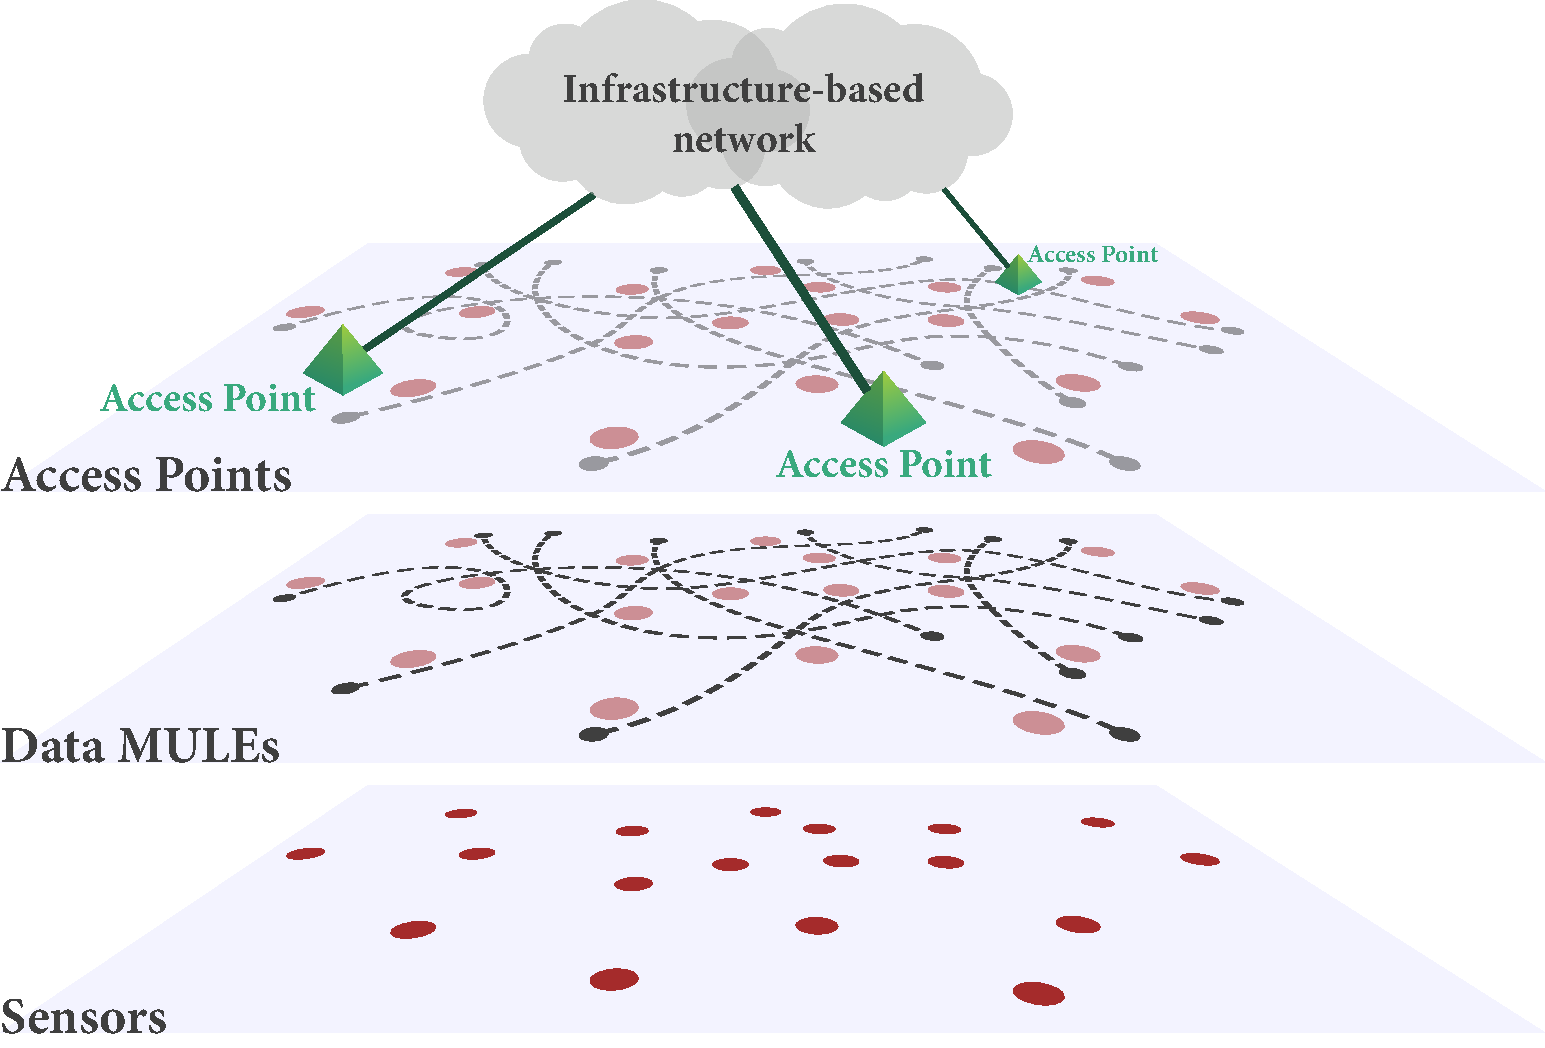
\includegraphics[width=0.7\textwidth]{figures/data-mules.pdf}
    \caption{Three-layered architecture for data \acrshortpl{mule}.}
    \label{fig:data-mules}
\end{figure}

ZebraNet\index{ZebraNet|bb} is was one of the first real-life deployment of a large-scale sensing platform. It monitors zebra wildlife by tracking their location history with collars they carry~\cite{juang2002energy}. The goal here is to learn more about the movements of zebras in Kenya. The location history logged in the collar is reported when the zebras come in range of base stations, which are either fixed or mobile, handheld by the researchers when they occasionally drive-by or fly-by to collect the data from the animals. The approach leverages two variations of the epidemic routing\index{Routing!Epidemic} algorithm to transmit the data from one zebra to another and increase the chances the data will be delivered to a base station. The authors considered a simple flooding algorithm, as well as a replication protocol based on the history of encounters. The epidemic protocol relies on a likelihood the zebra will come in range with the base station. The likelihood is estimated from the past successes at transferring data to the base station. Upon a contact with another zebra, if the likelihood of the other zebra is higher, then the data is relayed. The likelihood is incremented whenever the zebra comes within range of the base station and is decremented after a given duration away from the range of the base station. The protocols rely on a delete-list sent by the base station to delete the remaining copies of the file once a file has been delivered. The authors ran simulations based on real movements of zebras and compared the performance of the different routing protocols in terms of delivery ratio and energy consumption of the collars. They show that the history-based protocol performs better than the simple epidemic protocol and the direct delivery protocol when the storage or the bandwidth of the contacts are constrained. While the epidemic protocol has the highest success rate when both resources are unlimited, it involves buffering at intermediate nodes, this protocol has the highest energy consumption.

Burrell~\etal study the deployment of sensor networks in vineyards~\cite{burrell2004vineyard}. The study investigates the deployment of sensors throughout the vineyard such that it can help the vineyard workers take decisions such as knowing when the temperature becomes low or when to harvest based on the kind of wine the vineyard manager intends to create. The authors raise the problem of power management as a primary issue and propose solutions to avoid to replace the batteries of the sensor too often. Based on ethnographic studies, the authors realized that the vineyard workers were often moving up and down the rows, making them good candidates to serve as data \acrshortpl{mule}. Equipped with wireless storage devices, the workers can collect the sensor data and transmit them to an access point located at the farm, where the workers eventually return. With this deployment, the vineyard manager get the necessary feedback to take effective decisions concerning the vineyard.

The \acrfull{emma} project aims at monitoring pollution using the movements of buses that are part of existing Public Transportation Networks~\cite{lahde2007practical}. Pollution sensors are mounted on buses that collect location-based data with the movements of the buses. The data is then transported by the buses as part of their route to stationary gateways. The gateways are placed in strategic locations, such as intersections to capture the trajectories of buses. The gateways also use the movements of buses to forward control messages to smart display panels around the city, which show the current pollutant concentrations or traffic information. In their paper, the authors show extensive analysis of the feasibility of such a system by performing experiments using vehicles equipped with 802.11b \acrshort{wlan} interfaces. The authors assess the feasibility of such a scheme by evaluating the performance of the wireless communication between vehicles driving at different speeds in terms of data rate and data delivery. They observed delays of several seconds, which is suitable for the target applications.

SeNDT (Sensor Networking with Delay Tolerance) is a system for water pollution and noise monitoring at a lake in the centre of the Republic of Ireland~\cite{mcdonald2007sensor}. Sensors are placed around the lake to capture the environmental measures. However, the area of the lake is too large such that the sensors can form a fully connected wireless ad hoc network. Since the lake is popular with anglers, the authors mounted wireless devices on their boats that they use to fish in the lake. The devices then collect the sensor data when the boats come near the sensors. Once collected, the data is transmitted to a central sink when the boats return to the boat house at the end of the anglers' trip. The collected data can tolerate some delays, as the boats are expected to pass regularly near the sensors without any fixed schedule.

More sophisticated sensing platforms have been proposed to enable collaboration among entities to generate or collect sensing data, such as CarTel~\cite{hull2006cartel} and BikeNet~\cite{eisenman2009bikenet}. CarTel\index{CarTel|bb} is a distributed sensor system that relies on mobile vehicles equipped with communication capabilities (\eg WiFi and Bluetooth) to provide a software platform for sensing applications~\cite{hull2006cartel}. The vehicles collect environmental data necessary for various applications such as road traffic monitoring (commute delays and congestion), air quality monitoring, road state monitoring, or geo-imaging by attaching cameras on the vehicles to capture location-tagged image. Thus, the vehicles act as data \Acrshortpl{mule} that generate or collect environmental data and transport it to access points. The CarTel system also relies on vehicle-to-vehicle communications to forward data from one vehicle to another. To this end, the authors leverage a delay-tolerant network stack, \acrfull{cafnet} that enables mobile data muling (with the \acrlong{mal}, \acrshort{mal}) and the forwarding of data across an intermittently connected network~\cite{chen2007cafnet}. However, while \acrshort{cafnet} can implement complex routing strategies, the actual implementation remains basic with the Direct Delivery strategy that waits for the vehicles to be in the vicinity of the destination node to forward the data. CarTel was deployed on six cars, running on a small scale in Boston and Seattle for over a year. The system was used to analyze commute times, analyze metropolitan Wi-Fi deployments, analyze road conditions (potholes), and for automotive diagnostics. Additionally, the authors note that, these vehicles can serve as ``delivery networks'' to transport data from remote sensor networks to remote Internet servers. 

BikeNet\index{BikeNet|bb} is another sensor system that runs on bikes equipped with sensors (\eg by using Body Area Networks worn by the people on bikes)~\cite{eisenman2009bikenet}. Similar to CarTel, the system provides a platform for sensing applications, such as user-targeted applications (\eg health and safety) or environmental data collection for pollution monitoring or collective mapping. To collect the sensor data, access points are either fixed or mobile, carried by the people on bikes (\eg smartphones). When outside of the transmission range of an access point, a ``muling exchange'' takes place between the mobile sensors to exchange data and mule it to an access point. In their implementation, the authors propose a simple muling protocol based on an advertisement-accept-data exchange to forward the data to other sensors. The data exchange implements a 3-SACK policy for reliability by resending the data three times in case the exchange fails. However, the authors implemented a one-degree replication mechanism, allowing the source to transfer a single copy of the data to another sensor using the muling protocol. Additionally, the authors did not consider any multi-hop muling, and prevent intermediate nodes to forward or replicate the data to other nodes. This strategy allows to maintain control over the number of copies of data in the system. 

\section{Taxonomy: Use a support infrastructure to help transport the data}
\label{sec:indirect-delivery}

The work of Davis \etal~\cite{davis2001wearable} is one of the first that introduced the idea of using a support infrastructure to increase the connectivity and performance of ad hoc networks. In particular, they use controllable nodes to bridge the connectivity gap between ``connected'' regions. Connected regions refer to geographical areas where nodes are mobile and thus can communicate with one another. The authors consider scenarios where mobile nodes are restricted to two pre-defined regions distant from one another. They proposed to use a special node called \textit{relay} whose movements are restricted along a horizontal line that crosses the two regions. The purpose of the relay is to pass the packets generated by the mobile nodes in one region to the mobile nodes in the other region. Additionally, the authors proposed to use fixed nodes that act as mailboxes to enhance the performance of the data transport. The mobile nodes drop-off their data to these fixed nodes and other mobile nodes pick it up later. With relay nodes, the mobile entities do not need to be in the same location at the same time to exchange the data. They only have to meet the same relay node at different times. In the following, we review the work related to the use of infrastructure that helps transporting the data to its destination. In a first part, we review the approaches that leverage dedicated controlled entities to transport data between locations. In a second part, we review the work where a fixed infrastructure is deployed to help relay the data from one entity to another. Finally, we review the work that use an infrastructure already deployed, such as postal services to transport the data over large distances.

% However, the authors did not study how to control the trajectory of the relay node to maximize the packet delivery rate or delay.

\subsection{Mobile relays for spatially asynchronous data exchanges}

In this section, we review the approaches that use dedicated entities as a supporting infrastructure to transport data between different places. These entities have controllable mobilities that provide hard guaranties, for instance the delivery delay of the data. They can act as message ferries~\cite{zhao2004message} to collect data produced by sensors in a sensor field (\eg in underwater networks~\cite{partan2007survey}), enhance the capacity of ad hoc networks by providing more opportunities to transfer data to the non-controllable mobile entities~\cite{zhao2004message,burns2005mv}, or bridge the connectivity between different mobile regions~\cite{davis2001wearable,zhou2013minimizing}. However, the deployment of such mobile relays requires a control algorithm to coordinate their trajectories, for instance to satisfy some target requirements. The mobility of these mobile relays can be further subdivided into two categories. On the one hand, a \textit{static trajectory} corresponds to a path followed by the dedicated entity that is pre-computed and does not change over time. On the other hand, a \textit{dynamic trajectory} refers to a path followed by the dedicated entity that can change dynamically, in order to satisfy specific requirements of the target application (\eg timely delivery or collection, or rate of delivery).

% While the movements of the mobile entities are structured and can be predictable using the DTN techniques mentioned previously, the ``carry'' phase of the mobile entities can be under-utilized.

\subsubsection{Static trajectory of the mobile relays}

In the initial work of Message Ferry\index{Message ferry|bb}~\cite{zhao2003message}, Zhao \etal propose to use dedicated mobile nodes whose trajectory can be controlled to increase the performance of networks of stationary nodes. The stationary nodes are far enough from each others to be able to communicate between each others, so the ferry acts as a relay to enable the communication among the nodes by picking up the messages at the source and carrying them to the destination. One problem the authors address is the route design in the case of a single message ferry. Each node can be both sources and destinations of data transfers. The authors assume that these data transfers are already known in advance, allowing to design a ferry route such that the bandwidth requirements of the nodes are satisfied. They formulate the ferry route design as an optimization problem, which they further divide into two sub-problems. The first one aims to minimize the average delay for all traffic generated by the nodes. With symmetric traffic, this problem reduces to the well-known Euclidean \acrfull{tsp}\index{Travel Salesman Problem (TSP)}, which is known to be NP-Hard~\cite{papadimitriou1977euclidean}. The authors propose to adapt local optimization techniques, namely 2H-opt~\cite{bentley1992fast} to optimize the average delay of the resulting route, instead of the route length (generally optimized when solving the \acrshort{tsp}). The second sub-problem extends the ferry route generated by the first sub-problem to meet the bandwidth requirements of the nodes. The authors formulate this sub-problem as  a linear programming model that minimizes the amount of route extension of the ferry to visit the nodes and satisfy their bandwidth requirements. The simulation show that the introduction of a ferry can improve the network bandwidth and delay compared to the epidemic routing protocol, in particular when nodes are extremely disconnected.

In an extension of~\cite{zhao2003message}, the authors of~\cite{bin2006message} propose a route design algorithm so that a single ferry can visit the mobile nodes without any online collaboration between the nodes and the ferry nor change the mobility of the nodes (as it is the case in~\cite{zhao2003message,zhao2004message}). To this end, this algorithm designs a ferry route such that the ferry repeatedly visits determined locations for determined durations. The route consists of an ordered set of way-points and waiting times at these way-points. This route, or tour, is repeatedly traversed by the ferry. The route is designed such that it guarantees the ferry to meet the nodes with a certain minimum pre-determined probability, each time the ferry takes the tour. The route design algorithm consists of the following two steps. In the first step, the algorithm determines the way-points among a set of candidate points and the corresponding waiting times at these way-points such that the ferry meets the other nodes with a given probability (either while moving or while waiting at a way-point). In the second step, the algorithm constructs a path from the way-points using an heuristic that minimizes the weighted sum of the waiting times and the total distance of selected way-points from the center of the region. With simulations of various synthetic mobility models, the authors show that the optimized route design algorithm performs better than other naive route design algorithms that use random mobility or the \acrshort{tsp} to design the ferry route.

The authors of~\cite{zhao2003message} propose ways to improve the efficiency of the initial message ferry scheme. In particular, they propose to improve the delay of the ferry route by using the local connectivity of nodes and introduce clustering techniques that form connected components. With this approach, the ferry only visits one node per cluster, the \textit{cluster head} and exclusively communicates with it. The cluster head is in charge of gathering the messages of the others nodes in the cluster and distributing the messages received from the ferry to them with legacy ad hoc routing protocols. The authors note that the cluster head can see a high load of messages to transfer when the cluster becomes larger. This improvement was followed up by the work of Tirta \textit{et al.}~\cite{tirta2004efficient}. The authors propose to use this clustering technique to collect sensor data in remote fields. Similarly to the discussion in~\cite{zhao2003message}, the authors propose to use cluster heads that act as an equivalent of mailboxes, or intermediary points of collect that gather sensor data from the other nodes of the same cluster. When the ferry comes in the cluster head's transmission range, it starts transferring the data it accumulated from the other sensor nodes in the cluster to the ferry. The authors focus on the impact of the route schedule on the buffer size of the cluster head, as well as the average data collection latency, given the accumulation rate of the sensor data at each cluster head and the properties of the ferry route (distance between each pair of nodes and transmission rate of data from the cluster head to the ferry). To this end, the authors propose three algorithms to schedule the route of the ferry to visit the cluster heads. With the round-robin schedule, the ferry visits each cluster head to collect data in a round-robin manner. The data-rate based schedule plans the route of the ferry such that the visit frequency of a cluster head is proportional to the aggregate data rate from all the nodes in the cluster. Finally, with the min-movement schedule, the ferry visits the cluster heads depending on the proportion of the aggregate data rate such that the distance traversed is reduced. For each schedule, the authors analytically deduce the conditions on the route characteristics to minimize the buffer requirements at the cluster heads, as well as the average sensor network latency. With simulations, the authors show that the Min-movement schedule has better energy efficiency than the other two because the movements of the ferry consume more energy than the transmission. However, the latency of the data is comparable with the round-robin and rate-based schedules, and lower compared to the min-movement schedule. 

Underwater network are sensors networks deployed in the oceans for long-term environmental monitoring or surveillance~\cite{partan2007survey,akyildiz2005underwater,dunbabin2006data}. Because of the cost of the underwater sensor nodes and the extent of the areas to monitor, the deployment of such networks is generally sparse, making it impossible to form an unpartitioned ad hoc network. Hence, these networks include \acrfullpl{auv} to carry out maintenance functions and transport sensor data between the sensor nodes in the partitions. These networks differ from terrestrial sensor networks because of the acoustic channel shared between the communications among the sensors and the \acrshortpl{auv}, and the navigation system of the \acrshortpl{auv}. This twofold utilization of the medium creates contentions, limiting its use. Dunbabin \textit{et al.}~\cite{dunbabin2006data} deployed a test underwater network in a pool with an \acrshort{auv} that plans its route to visit known locations of stationary sensor nodes. The algorithm proposed by the authors consists in computing a tour for the \acrshort{auv} such that it visits all the sensor nodes. This algorithm is based on the \acrshort{tsp} and minimizes the distance traveled between two successive sensor nodes to limit significant errors due to uncertain locations of the sensor nodes. Briefly, a tour consists in travelling to the next sensor node using visual odometry, establishing a connection with the node (\eg optical or acoustic connection) once the sensor has been visually located. The \acrshort{auv} remains close to the sensor node until the transfer is over, at which point, the \acrshort{auv} begin traveling to the next sensor node. The \acrshort{auv} receives commands from a central gateway buoy~\cite{marn2005evolution} through a low bitrate channel. The \acrshort{auv} also uses a high-bitrate channel to send the data collected from the underwater sensors to the buoy.

The approaches we reviewed so far are applicable to the route design of a single controllable entity that follows a static trajectory (\eg to visit locations to exchange data from sensor deployed over an area of interest). In the following, we review approaches that tackle the challenges of having multiple controllable entities. Bringing more controllable entities increase the overall performance of the network (\eg in terms of capacity and latency), but raises significant challenges when it comes to design the route of the controllable entities and enable the communication among the entities.
% Such challenges include the route design of each entity to optimize given performance metrics, and the communication among the entities. 

One of the first work that considered multiple entities is an extension of the message ferry\index{Message ferry} scheme~\cite{zhao2003message,zhao2004message}. In this work~\cite{zhao2005controlling}, the authors propose different route design algorithms for multiple ferries to deliver data in networks of stationary nodes. The ferry route design algorithms aim satisfy the bandwidth requirements, while minimizing the weighted average data delivery delay in the network, where each traffic between two nodes is weighted to account for the relative importance of the data traffic. The authors note that, despite the cost, adding more ferries improves the network capacity and overall performance, as the ferries can cover larger distances, handle more traffic load, and provide better reliability in case of ferry failure. The authors propose a comprehensive work and consider multiple possible ferry interactions, with either no interactions, direct interactions, or indirect interactions. In the case of no interactions between the ferries, the authors propose to design a single route followed by all the ferries with the same speed and different timings, allowing each node to communicate with all the ferries. The route design follows reduces to the Traveling Salesman Problem, which is NP-Hard. The heuristic proposed by the authors is the same as~\cite{zhao2003message} and uses local optimization techniques that minimize the weighted average delay, coupled with route extensions to meet the bandwidth requirements of the static nodes. Still in the case of no interactions between the ferries, the authors propose another algorithm to design multiple routes followed by the ferries instead of a single route. Since the data is not relayed by the ferries, the routes must accommodate all the bandwidth requirements of each node visited by the ferry on the route. The algorithm is a greedy heuristic that assigns nodes to ferries and balances the traffic load among the routes by shortening or extending them such that the estimated weighted delay of the data traffic among the nodes is minimized. In this scenario, two nodes that communicate together cannot be served by two different ferries. To overcome the constraints introduced with the bandwidth requirements, the authors propose to relay data between ferries that follow different routes. In the case of direct interactions, the data is relayed by directly between the ferries at a point of intersection of their route. The ferry routes must be synchronized for two ferries to meet each other. In the case of indirect interactions, the data is relayed by static nodes that temporarily stores data. These nodes are similar to throwboxes since they relay data between ferries on different routes. The nodes are placed at locations where ferry routes intersect such that the estimated weighted delay introduced previously is minimized. In both of these interactions, the route design algorithm minimizes the number of ferry hops. In their evaluation of the different route design algorithms, the authors show that the multiple route algorithm with no interactions between the ferries performs the best in terms of delivery delay, in particular when the traffic load is high or the number of ferries is large. The algorithm with ferry synchronization performs the worst since it increases significantly the route route taken by the data. finally, when the load is high, the two algorithms with direct or indirect interaction perform the same as the single route algorithm in terms of delivery delay, since relaying data further increases the traffic load.

Tekdas~\etal propose to use mobile robots in the context of wireless sensor networks to move close to the sensor nodes and collect the data~\cite{tekdas2009using}. Similar to the use of data \acrshortpl{mule} (refer to Section~\ref{sec:data-mules}), the use of robots offers multiple advantages over using relay points that allow for multiple-hop data collection. Since the robots can move close to the sensor nodes, the quality of the link is high enough so that few retransmission are needed. Furthermore, the sensor node can reduce its radio transmission power, allowing to reduce the energy consumption. In this paper, the authors focus on the energy savings achieved by the introduction of mobile robots. They review techniques to wake up the sensor nodes when the robot comes close such that the nodes can save some energy when they are idle. They also review techniques for the robots to self-localize and to locate the sensor nodes when their position is not known in advance. Additionally, they authors give different approaches to design static routes for one or multiple robots. In the case of a single robot, one can use an instance of the \acrshort{tsp} that gives the shortest route to visit all the sensor nodes. In the case of multiple robots, one can use the $k$-\acrshort{tsp}, which finds $k$ tours where the largest of the $k$ tours is minimized. Finally, the authors describe a proof of concept with 12 sensor nodes and up to three robots supposed to visit the sensor nodes to aggregate their data. They performs various simulations with varying number of robots that show the energy consumption of the sensor nodes and the delay to collect the sensor data. The introduction of the mobile robots allows significant energy savings at the sensor nodes from 1mW to 0.003mW since the robots come close to the sensors to transfer data, which requires limited transmission power and less transmission attempts.

More recently, pigeon networks\index{Pigeon network} introduced \textit{pigeons} as a certain type of message ferries~\cite{zhou2013minimizing}. While both pigeons and message ferries are controlled, the main difference between the original message ferries and the pigeons is that each pigeon is dedicated to a ``foreign host'' (\ie a destination node) and travels between a ``home host'' (\ie a gateway) to this host on a dedicated route. Pigeon networks is then a generalization of real-life applications such as KioskNet or DakNet that both use buses (pigeons) to connect an Internet gateway (home host) to rural kiosks (foreign host). However, in a pigeon network, the pigeons are controlled and repeatedly visit the foreign hosts to collect the data they continuously generate. While the sources of the data can be different, the destination is always the home host. Firstly, the authors propose an exact optimization algorithm to obtain the optimal path to visit all the foreign hosts of the network while minimizing the average delay of the generated messages. This exact optimization algorithm is valid for small-scale network of a few nodes but becomes intractable when the scale of the network increases. To this end, the authors propose a geographical partitioning-based method that relies on the divide-and-conquer idea. They prove the lower-bound and upper-bound of the method and show that the designed routes allows for delays as low as 50\% less compared to the non-partitioning strategy proposed in~\cite{zhao2005controlling}. 

\subsubsection{Dynamic relaying of the data}

% Need to have global state of the network: either by having a centralized controller that maintains the holistic state of the network (traffic demands, locations and current movements of the controlled entities).

Li and Rus~\cite{li2000sending} is one of the pioneer work that studied the possibility of dynamically modifying the trajectories of mobile nodes in disconnected mobile ad hoc networks. This avoids the need to wait for a connection between the source and destination that may never become available. Given a known communication between two hosts, the authors developed algorithms that determine the routing path to send data. The algorithms minimize the modifications of the trajectories of the nodes and minimizes the delivery delay of the data on the determined path. The algorithms are presented under two assumptions, whether the movements of the nodes in the system are known or not. However, in this work, the hosts only move to form a multi-hop wireless routing path and do not actually carry the data from one host to the other. 

In one of original message ferry work~\cite{zhao2004message}, the authors proposed another approach called the \acrfull{nimf}\index{Message ferry!Node-Initiated Message Ferry (NIMF)} where the nodes proactively move close to the ferry. The ferry move around the area according to a specific route (where nodes are more likely to be). The ferry movements are known by the other nodes, for instance with the position of the ferry periodically broadcasted by the ferry or through an out-of-band control channel. Since the nodes must detour from their intended path to meet the ferry, the performance of the tasks assigned to the nodes can be degraded. The trajectory control of the nodes minimizes the message drop (caused by long delivery delay or buffer overflow) while limiting the detour made by the nodes. To this end, the authors consider a \acrfull{wtp} that represents the proportion of time the node works on its assigned tasks. If the ferry comes close to the node and the  current \acrshort{wtp} is below a defined threshold, the node can proactively make a detour to meet the ferry and exchange messages with it. With higher threshold, the message delivery rate degrades, as fewer nodes make a detour to meet the ferry. The simulations conducted in the paper show that the message ferry scheme yields significant improvements compared to the epidemic routing in terms of data delivery rate and delay, and energy consumption. 

In the \acrfull{fimf}\index{Message ferry!Ferry-Initiated Message Ferry (FIMF)} approach proposed by~\cite{zhao2004message}, the ferry proactively moves to meet with the nodes, instead of the nodes themselves, . Initially, the ferry follows a predefined route and broadcasts its position to the nodes over a long-range channel. When a node wants to send data, it generates a service request and transmits it to the ferry, along with its location. The ferry then detours from its route to meet the node, which periodically sends its location in case it moves from its original position. Once the ferry and the node are with the range of short-range radio, they begin exchanging data. After completing the data exchange with the node, the ferry moves back to its default route. The default of the ferry is designed to maximize the chance that the ferry is close to nodes and be in the range of their long-range radio. In this paper, the ferry follows a route which scans row by row the cells that divide the area of interest. The authors address the scheduling of multiple service requests received at a ferry. Each time the ferry receives a service request or a position update from a node, it computes a new route to meet the new node, in addition of the other nodes with pending service requests. The goal of the route computation is to minimize the expected data drops, either by buffer overflow or timeout. The route design reduces to a Minimum Latency Problem which is NP-Hard~\cite{blum1994minimum}. The authors develop the two following heuristics to make the problem tractable. With the nearest neighbor heuristic, the ferry always visits the closest node after it finishes meeting with a node. With the traffic-aware heuristic, the ferry computes the new route with the local optimization 2H-opt technique used to solve the TSP such that it minimizes the expected data drop. Similarly to the \acrshort{nimf} approach, the use of the ferry leads to significant improvements of the performance over the epidemic routing. The \acrshort{fimf} scheme has overall better data delivery and delay compared to the \acrshort{nimf} scheme, in particular when the buffer size of the ferry is low. However, the \acrshort{nimf} scheme achieves better energy efficiency because the nodes do not need to send control messages to the ferry. 

Burns~\etal~\cite{burns2005mv} introduced multiple autonomous agents to improve the network performance when the movement patterns of the participants do not match the bandwidth requirements of the data transfers. These agents dynamically adapt their movements according to the perceived conditions of the network and according to multiple objectives. The authors show that the problem of determining the optimal location for the agents is NP-hard~\cite{burns2008mora} by reducing the dial-a-ride problem\index{Dial-a-ride problem}~\cite{savelsbergh1985local} to their problem. Since the movements of the agents are determined locally in a distributed manner, the conditions of the network are maintained at each agent and include the list of carried packets for each participant and the timestamps of the last encounters. This information is exchanged and updated among the autonomous agents whenever they encounter one another. This information allows each agent to have an approximate global model of the network and take online and local decisions to improve the performance of the network given a set of objectives. Given static nodes with bandwidth requirements, the authors considered a set of four objectives to optimize: (1) maximize the \textit{total bandwidth} that refers the total number of messages in the network at a given point in time, (2) maximize the \textit{unique bandwidth} that captures the total number of unique messages in the network, without taking into account the replicas, (3) minimize the \textit{message latency} that refers to the average duration it takes to deliver a message, and (4) minimize the \textit{peer latency}, which captures the average duration since a node was last visited by an agent. The movement of the autonomous agents must optimize the given set of performance metrics. To this end, the authors propose to use two multi-objective techniques borrowed from robotics to balance the metrics, which are dependent on each other. The first technique relies on the nullspace composition, which uses a hierarchy of metrics to optimize such that the optimization of lower metrics are within the nullspace of the higher metrics. In other words, the optimization of those lower metrics does not affect the performance of the higher metrics. The authors choose an arbitrary order of the performance metrics based on observations they made and proceed to the nullspace composition of the metrics. The second technique is based on a subsumption approach. This approach differs from the nullspace technique in that it prioritizes the ordered metrics and optimizes them successively, starting from the higher ones, each up to a given performance threshold. In their simulations, the authors show that the nullspace approach outperfoms the subsumption one when the number of agents is limited. With more agents available, the two approaches become similar. They also show that the addition of agents significantly increases the performance of the network in both the delivery rate and the delivery delay compared to the sole use of epidemic protocols. In extensions of their work~\cite{burns2008mora,burns2006autonomous}, the authors propose the same algorithm that determines the route of the autonomous agents with nodes that are mobile, contrary to their first work that considered static nodes. In this case, the location of the nodes are known to the agents with the global state information disseminated in the network. One limitation of the approach is that the agents do not predict the future positions of the nodes; they only know their last positions advertised. 

The authors of~\cite{mansy2011deficit} revisited their original work on message ferry to take non-uniform distances and data rates of the nodes in the network. To this end, they propose to schedule the message ferry route to allow unequal visit frequencies at the nodes. The scheduling algorithm uses the \acrfull{drr} technique introduced in~\cite{shreedhar1995efficient}. With this approach, nodes with higher data rates get better chances to be visited by the ferry. The authors propose a heuristic algorithm to decide the next node to visit. Each node has credits, which are based on the visit history and the last meeting with the ferry. The ferry then chooses the node with the highest credits among the nodes least recently visited within a certain distance from its current position. Once the ferry has visited the node, its credits are set to zero. At the end of each round, the credits of the nodes are increased, with more credits allocated to nodes with higher rates. The authors then evaluate the performance of the heuristic against a standard route designed with the \acrshort{tsp} algorithm. As expected, the DRR-based route performs better than the TSP route, especially for non-uniform traffic.

\Acrfullpl{uav}, also called \acrfullpl{mav}\index{Micro Aerial Vehicle (MAV)} are more an more used in Search and Rescue missions~\cite{asadpour2016route,asadpour2013now,asadpour2014micro}. These missions are time-critical and necessitate to record images and videos of the area under consideration. Fleets of \Acrshortpl{mav} can hover over the areas and record them with on-board cameras and send the recordings back to the mission headquarters (a ground station). The challenge in this context is the timely delivery of data from the \Acrshortpl{mav} to a ground station. Since the \Acrshortpl{mav} are generally deployed in a sparse environment, ad hoc communications are not feasible, either among the flying \Acrshortpl{mav}, or between the \Acrshortpl{mav} and the ground station. However, since the \Acrshortpl{mav} are flying robots, one can control their movements to actively improve the link conditions by decreasing the distance between the two communicating \Acrshortpl{mav}. To this end, two communication channels are needed to enable data-intensive application (such as video recording): a long-range low-throughput control channel for telemetry and control data with the ground station and a high-throughput channel to establish communication among the \Acrshortpl{mav} and the ground station. The \Acrshortpl{mav} use two types of actions to establish connectivity: \textit{relaying} the data by forwarding it to another \Acrshort{mav} or the ground station according to a routing algorithm, and ferrying to physically carry the data and transmit it to the wireless network. Thus, there are two types of MAVs: the hovering \Acrshortpl{mav} in charge of the recording for instance, and the ferry \Acrshortpl{mav} that provide connectivity between the \Acrshortpl{mav} and the ground station. Under the assumptions of the authors, the paths of the ferry \Acrshortpl{mav} can be determined in a deterministic way, since the data traffic is asymmetric (from the \Acrshortpl{mav} to the ground station). The ferry \Acrshortpl{mav} move back and forth between the hovering \Acrshortpl{mav} and the ground station to collect data and deliver it. In the field experiments and the simulations conducted in~\cite{asadpour2016route}, the authors arbitrarily assign pre-defined routes for the ferry \Acrshortpl{mav} such that they connect the hovering \Acrshortpl{mav} and the ground station. Further, the authors propose a location-aware geo-routing algorithms that decide whether to forward or carry data. The algorithm chooses the forward data along the spatially shortest path to the destination if there is such a path or if the neighbor is spatially closer to the destination. Otherwise, the algorithm decides to keep the data and carry it on the \Acrshortpl{mav} until it encounters the destination or a more suitable \Acrshort{mav} (\eg a ferry \Acrshort{mav}). The algorithm relies on a estimate of the future proximity of the \Acrshortpl{mav} to the destination, calculated using a linear mobility model of the \Acrshortpl{mav} that predicts the future positions in the near future. The authors evaluate the benefits of the ferries and conclude that the use of ferries improves the performance of the \Acrshort{mav} fleet in terms of both the delivery delay and the delivery ratio of the data.

\subsection{Fixed relays for temporally asynchronous data exchanges}
\label{sec:fixed-relays}

In the Infostation model\index{Infostation|bb}, mobile entities can connect to access multiple points distributed over a geographical area~\cite{goodman1997infostations}. Infostations are devices that offer high capacity connectivity to entities within their vicinity. Since the entities are mobile and because of the lack of coverage provided by the high density of nodes, the resulting connectivity is intermittent. This model thus trades connectivity for capacity by exploiting the mobility of the entities. With the Shared Wireless Infostation Model, Small and Haas propose a model to trade-off capacity and delay based on both the Infostation model and epidemic routing~\cite{small2003shared}. In particular, the authors consider the case of whale monitoring, where radio-tagged whales continuously collect biological and environmental data. Contrary to previous approaches where the data was sent to LEO satellites when the whale surface, the approach proposed by the authors leverages Infostations to ``offload'' or collect the monitoring data locally stored on the whales' tags when they surface. Once the data is offloaded to an Infostation, the memory of the tag is cleared. The authors study the impact of the placement of the Infostations at fixed locations (typically on buoys) where whales usually surface, as well as on mobile locations (here, on  seabirds). The epidemic protocol is used to exchange monitoring data when the whales are grouped together. To avoid having too many copies of the same file in the network, the authors propose to use an infectious disease model that will ``infect'' the whale with a data given a probability, if not already infected. This probability is chosen such that it is equal to the probability that the data will be offloaded within a target duration since its generation. With simulations, the authors show that the epidemic protocol allows to reduce significantly the delivery delay of the data compared to the sole use of the Infostation. They also observe trade-offs such as reliability vs storage space both when using the epidemic protocol to replicate data between whales and when adding more whales to carry the data.

Instead of relying on random node mobility, Zhao~\etal proposed the use of small inexpensive battery-powered devices equipped with storage and wireless interfaces called \textit{throwboxes}\index{Throwboxes|bb}~\cite{zhao2006capacity}. Throwboxes enhance the delivery likelihood of mobile ad hoc networks by increasing the contact opportunities when placed at strategic locations. A mobile entity can offload the data it carries to the closest throwbox where it will be temporarily stored until transmitted later to another mobile node. The authors investigate the gain on the overall achieved throughput when deploying throwboxes. To this end, they propose three different deployments based on the different knowledge of the traffic matrix and the future contacts among the entities and the candidate locations of throwboxes, which are located at the center of cells that divide the geographic area. The authors model the joint deployment and routing with linear programing models. Since these problems are NP-Hard, the authors give greedy algorithms that make the problem tractable. Further, they propose three routing approaches to route data through the network that consists of the allocated throwboxes and the mobile entities. In the first approach, the data is forwarded using the Epidemic protocol, and copies are generated when two mobile entities are in contact together or when a mobile entity is in contact with a throwbox. This strategy has limited performance because of the poor utilization of the resources resulting from the flooding of messages, which leads to message drops. In the second approach, the authors propose to use multi-path routing, where messages are not replicated and are routed along different paths. The routing and the chosen paths are optimized by the model and the heuristic they propose. This approach yields the best results in terms of delivery delay and delivery ratio, since the resources are fully utilized. Finally, the third approach considers only one path from the source to the destination, which results in poor utilization of the resources. While this approach has lower delivery ratios than the multi-path routing approach, it allows reducing the delivery delay, as only the shortest path is used to transport the data to its destination. 

Banerjee \etal extended the original work on throwboxes\index{Throwboxes} and proposed an architecture that trades the power consumption and the amount of data forwarded by the throwboxes. Power saving of the throwboxes is necessary, as it increases the lifetime of the throwbox. Adding solar power allows potential infinite utilization, if the energy consumption is less than the energy gain. One solution is to turn the throwboxes on and off intermittently when no contacts are detected. According to the authors, the primary source of energy consumption is the neighbor discovery: turning the throwbox on and searching for potential contacts is costly in terms of energy. To this end, the authors propose an approach that provides efficient neighbor discovery that relies on the mobility detection of other nodes. They separate the neighbor discovery task from the data transfer tasks, which requires high-bandwidth connections. A long-range channel efficiently listens for contacts (duty-cycle), while a high-bandwidth radio remains asleep. If the contact proves to be fruitful, the high-bandwidth radio wakes up and begins the data transfer with the node. A throwbox estimates whether a contact will be fruitful by predicting the future mobility of the node using a Markovian model based on the past positions of the node broadcasted to the throwbox using a long-range channel. If the throwbox estimates that the node will come within the range of the high-bandwidth radio, it determines whether the contact represents an opportunity worth considering. To this end, the authors propose a scheduler based on a token-bucket approach that generates energy tokens at the rate of the average power constraint. Based on the current amount of tokens available, the scheduler determine whether it should accommodate this connection or the next one based on the inter-arrival rate and mean size of the last connections. The authors implemented prototype throwboxes with the UMass DieselNet\index{DieselNet|bb} testbed~\cite{burgess2006maxprop}. DieselNet is a vehicular network that consists in 40 buses equipped with WiFi capabilities serving the surrounding area of UMass Amherst campus. The testbed was used to measure and model the intermittent connectivity between buses, as well as to evaluate MaxProp\index{Routing!MaxProp}, a routing protocol designed specifically for delay-tolerant networks. In the case of MaxProp, data forwarding results of local decisions made by each bus according to a \textit{Delivery Likelihood} estimation based on history information about past meetings with other buses. They conducted evaluations using MaxProp to route data across the nodes and they compare the performance of their system with other systems to wake up the network interfaces in terms of energy efficiency, delivery delay, and delivery rate. They show that their system performs better than the other schedulers in terms of energy efficiency and almost as well as an alway-on throwbox in terms of delivery rate and delay, while saving significantly more energy and allowing to last 31 times longer on the same battery.

Dead Drop\index{Dead Drop|bb}\footnote{\url{http://deaddrops.com/}} is an art project that uses USB sticks placed at different locations in cities (\eg on the walls of buildings). The USB sticks allow for anonymous peer-to-peer file sharing where people can drop off  data and other people can pick it up. Multiple approaches propose to use these dead drops (equipped with wireless communication capabilities) as intermediary points to relay data from one entity to another~\cite{chawathe2006inter,chawathe2008using,lok2009data}. In these works, a dead drop is a wireless transceiver, placed at an intersection, that stores data transmitted by passing vehicles and transmits them to vehicles that pass later. In~\cite{chawathe2006inter}, Chawathe proposes to use dead drops to disseminate data using the opportunistic movements of vehicles to transport data from one dead drop to the other. In particular, the author is interested in the placement of the dead drops such that it provides the required connectivity between flows of vehicles traveling different routes of interest at minimum deployment cost. To this end, the author model the placement of dead drop as a variant of a minimum-weight $k$-set cover problem, which is NP-Hard. Hence, the author present a greedy polynomial-time algorithm to place the dead drops, given the min-cost and connectivity constraints. In~\cite{chawathe2008using}, the same author as the previous work evaluated the dissemination properties of such a network of dead drops with varying traffic densities (\eg flows of vehicles traveling between the dead drops) and varying number of dead drops in the city of Falmouth, MA. Compared to the sole use of vehicle-to-vehicle communications, the use of dead drops helps increasing the dissemination of the data in the network of dead drops.

The authors of~\cite{ibrahim2009analysis} propose an analytical framework to evaluate the packet delivery delay and the number of replicas needed when transmitting data in ad hoc networks equipped with relay nodes. The framework is based on a Markovian model of the network where the successive contact opportunities between two mobile entities or between an entity and a relay node are represented by a Poisson process. The authors propose different relaying strategies with different forwarding rules whether the node is the source or the destination of the data, or a relay node either between nodes or throwboxes. They compare them in terms of delivery delay and number of copies generated per message. Allowing more forwarding interaction among both the mobile entities and the relay nodes reduces the delivery delay of the messages, but increases the number of copies generated per message. However, restricting the forwarding to the sole interactions between the mobile entities and the relay nodes yields poor performance in terms of delivery delay and number of copies generated, as the source and destination must come close to a relay node to either transmit or receive the data.

Banerjee~\etal study mobile networks enhanced with a supporting infrastructure to relay the data between different mobile entities~\cite{banerjee2008relays}. Specifically, the authors compare the deployment of three different kinds of static nodes: (i) relay nodes that act as throwboxes, (ii) mesh nodes that are connected together by long range wireless links, and (iii) base stations connected together by an infrastructure network that act as Infostations. The authors deployed relay nodes in a small vehicular network and measured the contacts between two vehicles, and a vehicle and a relay node. They then performed simulations based on the collected measures with both uniform and geographically-weighted placement of the stationary nodes, as well as different forwarding strategies, including 2-hop (no mobile-to-mobile communications), random Epidemic (to limit the number of copies generated by message), and RAPID~\cite{balasubramanian2007dtn,balasubramanian2010replication}. RAPID\index{Routing!RAPID} is a forwarding protocol for delay-tolerant protocols that treats routing as a resource allocation protocols and determines the degree of replication of a message by estimating the suitability of a contact. The authors observe that the deployment of a small number of stationary nodes allows a large decrease of the expected delivery delay. Deploying $x$ base stations allows reducing the average packet delay by a factor of two. The same reduction requires $2x$ mesh nodes and $5x$ relays. Additionally, the authors propose an analytical model applicable for large-scale networks.

KioskNet\index{KioskNet|bb} is a system very similar to DakNet~\cite{seth2006low,guo2007very,guo2011design}. However, the authors of KioskNet provide a generic architecture targeting distributed applications that allow disconnections and long delays. These applications rely on rural kiosks, which provide several services, including birth and death certificates, bill collection, email, and land records. Satellite or dial-up landline communications generally connect the kiosks to the Internet. However, these connections are expensive and not reliable.  The goal of KioskNet is to provide a low-cost alternative to connect rural kiosks together. Similar to DakNet, the architecture consists of the kiosks that act as gateways, and vehicles (\eg buses, motorcycles, trains, and even bullock carts) that have predictable movements between the kiosks. Both components are equipped with wireless connectivity and storage. The movements of the vehicles between the kiosks creates a mechanical backhaul\index{Mechanical backhaul} that transport data between an Internet gateway and the kiosks. The authors focus on the control plane of the system, as routing errors at kiosks can incur delays of several days. To this end, they discussed the use of different routing protocols to forward the data to its destination using routers located at the kiosks. The protocols discussed include flooding (does not scale), reverse-path forwarding (fragile in case of failures), and link-state routing. For the latter protocol, logical links connect the routers and correspond to the movements of the vehicles between the routers. The authors consider using the expected delay between two kiosks as the link weight. The shortest path algorithm is used to populate the forwarding tables at the nodes.  and they also discuss on how the weights can be updated in case the buses are delayed. Additionally, the authors overview other aspects related to the system, such as the security, naming, and implementation. The authors implemented a prototype in India and Ghana with a simplified system architecture. The performance they obtained were the same as the one obtained with DakNet. Following the efforts of KioskNet, Demmer and Fall propose \acrfull{dtlsr} to adapt \acrfull{ls} routing to delay-tolerant networks~\cite{demmer2007dtlsr}. In particular, the authors propose to modify the \acrfullpl{lsa} to report the connectivity status of the nodes in the network. With legacy LS protocols, if a link to a node is unavailable at the time the \Acrshort{lsa} is computed, the protocol considers the node as unreachable. However, with delay-tolerant networks, the node may be connected at a later time: the lack of recent contact with a neighbor does not imply that the connectivity between the two nodes is unavailable. To this end, \acrshortpl{lsa} are sent with long lifetimes to take the changes in the connectivity into account. Additionally, each node calculates an estimate of the expected delay to forward a message over the given link. The data is then routed using a shortest-path algorithm (\eg Dijkstra) such that the estimated expected delay is minimized. With experiments conducted on buses traveling between kiosks in the region of Tamil Nadu, India, the authors show that \Acrshort{dtlsr} performs better than traditional link state routing protocols with shorter lifetimes, in terms of delivery ratio and delivery rates. Additionally, the authors compare the use of wireless links connecting the different kiosks with buses transporting the data. The observed that the implementation of the protocol on buses leads to better performance compared to the wireless links. 

Zarafshan-Araki~\etal proposed TrainNet\index{TrainNet|bb} to transport delay-tolerant data on trains, which also act as a mechanical backhaul\index{Mechanical backhaul}~\cite{zarafshan2010trainnet}. In TrainNet, trains and stations are equipped with large data storage. The trains pickup data at one station and deliver it at another station on their route. For instance, upon a train arrival at a train station, the data can be handled by a staff member of the rail network who will swap the hard drives at the station with the ones on the train. The authors focus on the scheduling of the data, as the train have limited storage available and only a limited amount of data can be exchanged at stations. In particular, the authors formulate the routing problem as a resource allocation problem and use different max-min fair algorithms to guarantee fair allocation of the resources to the different competing flows. The algorithm maximizes the throughput and hard drive utilization, while minimizing the delay and data losses. With simulations on a small network of four stations and conservative hard drive sizes, the authors observed a throughput of 1.4~Gbps, which is equivalent to the throughput of a fiber land line connection.

\subsection{Third-party carriers to transport the data}

With the explosion of the Internet volumes over the past few years, the idea of offloading data from the Internet has become more relevant. The potential of offloading is well illustrated by Andrew Tanenbaum\index{Tanenbaum|bb}~\cite{tanenbaum2003computer}:
\begin{quote}
    \textit{Never underestimate the bandwidth of a station wagon full of tapes hurtling down the highway.}
\end{quote}

However, the idea of transferring data by physically moving removable storage media is not new and is commonly referred as SneakerNet\index{SneakerNet|bb}~\cite{patterson2003conversation}. RFC 1149 (and its later improvements) specifies an experimental method to transmit IP datagrams using avian carriers~\cite{rfc1149}. Although suited in very specific scenarios, this solution becomes unfeasible in large-scale networks due to the resulting high delay and low throughput. Additionally, the number of pigeons grows linearly with the number of data transfers, as one pigeon is needed for each transfer. Some implementations of the protocol lead
\begin{wrapfigure}[11]{o}[0.7\marginparwidth]{5cm}
    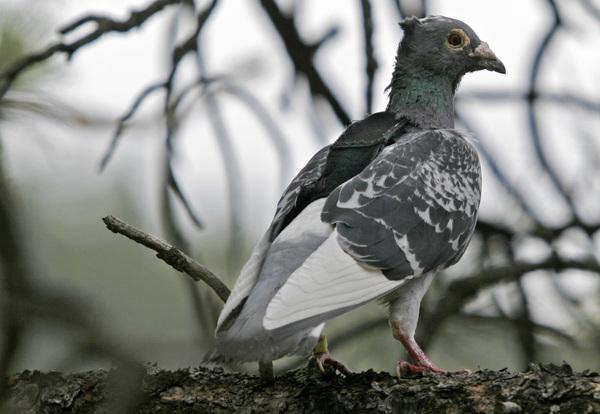
\includegraphics[width=4.9cm]{figures/pigeon.jpg}
    \caption{A pigeon equipped with a small backpack to carry an SD card.}
    \label{fig:pigeon}
\end{wrapfigure}
to large losses (over 55\% of the datagrams were lost during the test phase) and variable delays of several hours when transporting the data over five kilometers. However, this solution has been used in real-life scenarios. For instance, some photographers used trained pigeons in remote regions to send pictures in a SD card over short distances\footnote{\url{http://origin.denverpost.com/opinion/ci_6209735}}. The pigeons were able to achieve a bandwidth comparable to a landline ADSL connection with few losses. 

The DOT (\textit{Data-Oriented Transfer}) project is an architecture for bulk data transfers~\cite{tolia2006architecture}. The architecture enables wired data transfers on infrastructure-based networks, as well as physical data transfers, for instance by physically carrying a USB stick from one computer to another. It provides APIs to transfer data either on wired medium or by physically carrying USB sticks. In their evaluations, the authors compare the use of a fast residential cable Internet link with the use of USB sticks to transfer data between the computers. The two computes are located five minutes away from each other. As expected, the total time to transfer the data is much lower using the USB sticks compared to using the Internet. 

Service providers can turn to third-party carriers to transport data over large distance such as postal services (\eg USPS, La Poste, FedEx, or UPS). Using these carriers avoids deploying and maintaining costly data transport infrastructure such as the ones we reviewed in the previous section, which are more suitable for long-lived data transfers. Postal services provide hard guarantees on the delivery duration of parcels, as well as on the shipping cost. The joint use the Internet and postal services for data transfers was first proposed by Wang~\etal~\cite{wang2004turning}. The authors propose Postmanet\index{Postmanet|bb}, a generic system that extends or complements the Internet and provides connectivity to areas in rural regions. The Postmanet channel is referred as a ``High Latency High Bandwidth'' channel (HLHB), which contrasts with ``Low Latency Low Bandwidth'' channels (LLLB) such as satellite or landline dial up connections. In particular, the authors propose to use the latter channel as a control channel to send control messages such as acknowledgments. The data is copied on DVDs and shipped in parcels to a remote Postmanet router that acts as a gateway, which, in turn, puts the received data at disposal to the remote users (\eg email or records). Multiple routing strategies are discussed in the paper. The first one is to use a central server that aggregates the data received from parcels and dispatches the data to the users by shipping it in parcels. While this strategy can incur unnecessary delays (\eg when the server is not located in a central location), it allows efficient sharing of data when data needs to be sent to multiple users (the central server then acts as a switch). The second strategy proposed by the authors is a peer-to-peer approach where the users send the data directly to one another. The shipping information of the users is known through a central controller using the LLLB channels. This strategy is more efficient in terms of shipping delays, however, it requires shipping and receiving many parcels, which can become costly for large-scale networks. The third strategy is a strategy that combines both previous strategies. Multiple distribution centers are distributed geographically and the users send the data to the closest center. However, the authors do not provide any quantitative comparison of the different routing strategies. 

Cho and Gupta proposed the Pandora (\textit{People and Networks Moving Data Around}) system, which makes a joint use of both the Internet and postal services for large-scale bulk transfers planning~\cite{cho2010new,cho2011budget}. The authors focus on the problem of satisfying a latency deadline, while minimizing the total cost of the transfer (which includes shipping and Internet costs). To this end, they leverage an overlay of the sites connected by shipping links and Internet links. Each logical link is represented by a capacity, cost and transit time. While an Internet link has constant attributes over time, shipping links have variable attribute values over time (\eg both the cost and transit time vary as a function of the level of service~---~Overnight, Two-day, Ground). The authors then formulate the flow and constraints on the overlay over time that takes into account dynamic and time-sensitive data movement. Since the formulation is NP-Hard, the authors derive an optimal solution based on a Time-Expanded Network of the overlay, which represents the possible flows on all edges and vertices of the network for the whole duration of the transfer. The flow problem using the Time-Expanded Network can only be solved as a Mixed Integer Programming Model since the edges have fixed costs, which makes it also NP-Hard. To make the problem tractable, the authors propose several optimizations of the attributes of the network, and use $\Delta$-condensed networks to find fast approximate solutions for the problem. These optimizations make the problem tractable for large-scale networks. finally, the authors evaluate the performance of the system for different transfers plannings. In every cases, the system outperforms the single use of the Internet or shipping method to transfer data. 

Laoutaris~\etal compared the actual cost of sending data using postal services with the cost of sending the same amount of data through an infrastructure-based network, as content providers operating several datacenter would do~\cite{laoutaris2009delay,laoutaris2013delay}. The data transfers target delay-tolerant bulk data, as the data produced by CERN's Large Hardon Collider that tolerate delay of a few hours to a few days. Such data transfers are currently serviced by expensive dedicated networks (\eg Large Hardon Collider Computing Grid) or by postal services using hard drives and disks. The authors propose strategies to schedule the data transfers over an \acrfull{isp} such that the cost of the transfer is minimized. In particular, they propose to benefit from the ``load valleys'' that happen during off-peak hours (\eg at night time) and when sending data is free because of the 95-percentile pricing scheme used by transit ISPs to charge their customers. To synchronize the non-coinciding off-peak hours of the different ISPs traversed by the data transfer, the authors perform Store-and Forward using an assisting storage node that buffers the data and delays the transfers to send it during subsequent load valleys. This intermediate storage is necessary for transfers that have at least 5 hours of time-zone difference. The authors compare the cost of this approach with the cost of sending the same amount of data using postal services. The results show that it is less expensive to use to postal services for individual shipments that occasionally happen (\eg short-lived transfers). However, in the case of a constant flow of data to transfer, shipping data is more expensive than sending it through an \acrshort{isp} using the delayed forwarding the authors propose.

Note that, the postal services are used in many commercial applications. For instance, Netflix\index{Netflix} offers a DVD rental service to its customers\footnote{\url{http://dvd.netflix.com/}}. Customers choose a DVD to rent and Netflix sends it through postal services. Customers may keep the DVD as long as they want, and must return it before renting another DVD. It has been reported that Netflix distributes more than 1.5 million DVDs a day\footnote{\url{ http://ir.netflix.com}}, accounting for a total aggregate bandwidth of more than 650 Gbps. 
\begin{wrapfigure}[11]{o}[0.7\marginparwidth]{4.4cm}
    \centering
    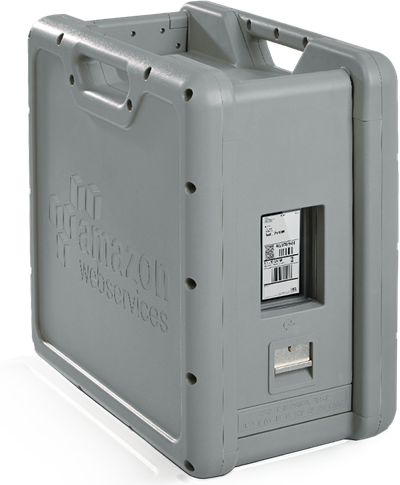
\includegraphics[width=3cm]{figures/Snowball.png}
    \caption{Amazon Snowball}
    \label{fig:snowball}
\end{wrapfigure}
% http://files.shareholder.com/downloads/NFLX/182838532x0x102020/5a5dc220-6f8b-4704-a380-2c81a3a37958/factsheet.pdf
Another examples are the recent services proposed by large cloud providers (\eg 
AWS Import/Export\index{Amazon Web Services (AWS)!Import/Export}\footnote{\url{http://aws.amazon.com/importexport}}, 
Microsoft Import/Export Service\footnote{\url{http://azure.microsoft.com/en-us/documentation/articles/storage-import-export-service/}} and more recently 
Google Offline Disk Import\footnote{\url{https://cloud.google.com/storage/docs/early-access}}). They allow their customers to ship hard drives containing their data to be uploaded to cloud storage, instead of using their own Internet connection that can be slow, in particular in the first mile of the transfer, at the access network. AWS launched the Amazon Snowball\index{Amazon Web Services (AWS)!Snowball} (shown in Figure~\ref{fig:snowball}), a portable ready-to-be-shipped appliance with a storage capacity of 50~TB that can accommodate transfers of several Petabytes (using multiple Snowball) to AWS servers. The appliance has an e-ink screen that displays the shipping label to be handled by shipping services such as UPS or FedEx\index{Postal services!FedEx}\index{Postal services!UPS}. Amazon compares this solution with transfers on common Internet connections. It takes less that one day to transfer 50~TB via a 10G connection. Conversely, it takes less than a week to ship a Snowball. However, most Internet connections cannot accommodate transfers of 10~Gbps. In Table~\ref{tab:truck-full-of-drives}, we show the number of days it takes to transfer 50~TB via typical Internet connections. Amazon Snowball compares to these Internet connections and can perform high-bandwidth transfers. With this appliance, Amazon customers trade speed for money, as renting a Snowball costs \$200 plus the shipping costs. Comparatively, leasing a dedicated line from a Tier 1 ISP (\eg Level 3) costs about \$1~-~\$2 per Mbps for a 10G port, which rounds up to \$10,000 for a fully utilized 10G port (including collocation and equipment leasing costs)\footnote{\url{http://drpeering.net/white-papers/Internet-Transit-Pricing-Historical-And-Projected.php}}. Therefore, as noted by Laoutaris \etal~\cite{laoutaris2009delay}, leasing an Amazon Snowball for a single transfer is more profitable than leasing a dedicated line for similar resulting bandwidth.

\begin{table}[h]
    \centering
    \begin{tabular}{|c|c|c|c|c|}
        \hline
         & \multicolumn{4}{c|}{Internet connection speed} \\
        \hline
        Utilization & 1Gbps & 500Mbps & 300Mbps & 150Mbps\\
        \hline
        25\% & 19 & 38 & 63 & 126 \\
        \hline
        50\% & 9 & 19 & 32 & 63 \\
        \hline
        75\% & 6 & 13 & 21 & 42 \\
        \hline
    \end{tabular}
    \caption{\textit{How fast is that truck full of drives?}~---~Numbers of days to transfer 50~TB via the Internet at typical utilizations. The table appeared on slides from Amazon Web Services.} 
    % \footnote{\url{http://www.slideshare.net/AmazonWebServices/aws-october-webinar-series-introducing-aws-import-export-snowball}}.}
    \label{tab:truck-full-of-drives}
\end{table}


\section{Summary and relationship with the thesis}
\label{sec:summary-relationship-related-work}